\PassOptionsToPackage{table}{xcolor}
\documentclass[a4paper,12pt]{article}
\usepackage[top=25mm, bottom=25mm, left=20mm, right=20mm]{geometry} 
\usepackage{fancyhdr}
\usepackage{graphicx}
\usepackage[table]{xcolor}
\usepackage{tikz}
\usetikzlibrary{arrows.meta, positioning}
\usepackage[utf8]{inputenc}
\usepackage{setspace}
\usepackage{multicol}
\usepackage{tabularx}
\usepackage{booktabs}
\usepackage{float}
\usepackage{subcaption}
\usepackage{chngcntr}
\usepackage{tocloft}
\tocloftpagestyle{clean}
\usepackage{titlesec}
\usepackage{amsmath,amssymb}
\usepackage{newtxtext,newtxmath}
\usepackage[hidelinks]{hyperref}
\usepackage{longtable}

% --- 1. TOC & LIST OF FIGURES / TABLES FORMATTING (TOCLOFT) ---
\counterwithin{table}{section}
\counterwithin{figure}{section}

\renewcommand{\contentsname}{TABLE OF CONTENTS}
\renewcommand{\cfttoctitlefont}{\hfill\Large\bfseries}
\renewcommand{\cftaftertoctitle}{\hfill\null\\[1.5em]\null\hfill\normalfont\normalsize Page\par\vspace{-0.5em}}

\renewcommand{\cftdotsep}{1.5}
\renewcommand{\cftsecleader}{\cftdotfill{\cftdotsep}}
\renewcommand{\cftsubsecleader}{\cftdotfill{\cftdotsep}}
\renewcommand{\cftsubsubsecleader}{\cftdotfill{\cftdotsep}}
\renewcommand{\cftfigleader}{\cftdotfill{\cftdotsep}}
\renewcommand{\cfttableader}{\cftdotfill{\cftdotsep}}

\renewcommand{\cftsecfont}{\normalfont\bfseries}
\renewcommand{\cftsecpagefont}{\normalfont}
\setlength{\cftsecindent}{0pt}
\setlength{\cftsecnumwidth}{0pt}
\setlength{\cftbeforesecskip}{6pt}

\renewcommand{\cftsubsecfont}{\normalfont}
\renewcommand{\cftsubsecpagefont}{\normalfont}
\setlength{\cftsubsecindent}{0.8cm}
\setlength{\cftsubsecnumwidth}{1.0cm}
\renewcommand{\cftsubsecaftersnum}{.}
\setlength{\cftbeforesubsecskip}{3pt}

\renewcommand{\listfigurename}{LIST OF FIGURES}
\renewcommand{\cftloftitlefont}{\hfill\Large\bfseries}
\renewcommand{\cftafterloftitle}{\hfill\null\\[1.5em]\null\hfill\normalfont\normalsize Page\par\vspace{-0.5em}}
\renewcommand{\cftfigpresnum}{\textbf{Figure }}
\renewcommand{\cftfigaftersnum}{:}
\setlength{\cftfignumwidth}{2.8cm}

\renewcommand{\listtablename}{LIST OF TABLES}
\renewcommand{\cftlottitlefont}{\hfill\Large\bfseries}
\renewcommand{\cftafterlottitle}{\hfill\null\\[1.5em]\null\hfill\normalfont\normalsize Page\par\vspace{-0.5em}}
\renewcommand{\cfttabpresnum}{\textbf{Table }}
\renewcommand{\cfttabaftersnum}{:}
\setlength{\cfttabnumwidth}{2.8cm}

% --- 2. PAGE STYLES ---

% Style A: Clean (TOC / Lists / Front Matter) - FULLY BLANK
\fancypagestyle{clean}{
    \fancyhf{}
    \renewcommand{\headrulewidth}{0pt}
    \renewcommand{\footrulewidth}{0pt}
    \fancyfoot{}
}

% Style B: Report Body (Continuation Pages & Chapter Opening)
\fancypagestyle{reportstyle}{
    \fancyhf{}
    \fancyhead[C]{\textbf{IntentCloud}}
    \fancyfoot[L]{\textbf{Dept of CST}}
    \fancyfoot[C]{}
    \fancyfoot[R]{\textbf{\thepage}}
    \renewcommand{\headrulewidth}{0.8pt}
    \renewcommand{\footrulewidth}{0.8pt}
}

% Style C: Section Start (Ensures Header and Footer stay intact)
\fancypagestyle{plain}{
    \fancyhf{}
    \fancyhead[C]{\textbf{IntentCloud}}
    \fancyfoot[L]{\textbf{Dept of CST}}
    \fancyfoot[C]{}
    \fancyfoot[R]{\textbf{\thepage}}
    \renewcommand{\headrulewidth}{0.8pt}   
    \renewcommand{\footrulewidth}{0.8pt} 
}

% --- 3. CUSTOM COMMAND FOR SECTIONS / CHAPTERS ---
\newcommand{\mysection}[1]{%
    \clearpage
    \refstepcounter{section}%
    \addcontentsline{toc}{section}{\textbf{CHAPTER \thesection\quad #1}}%
    \sectionmark{#1}%
    \thispagestyle{reportstyle}%
    \vspace*{0.2cm}%
    \noindent{\textbf{\Large CHAPTER \thesection}}\par
    \vspace{0.8cm}
    {\centering\textbf{\Large\MakeUppercase{#1}}\par}
    \vspace{1.2cm}
}

\onehalfspacing

\begin{document}

% --- FRONT MATTER (PAGES 1-5 WITHOUT MARGIN / BORDER) ---
\pagestyle{empty}
\pagenumbering{gobble} % Hides page numbers for front matter

% 1. TITLE PAGE
\begin{titlepage}
\thispagestyle{empty}
\begin{center}
    % Header Logos - Using minipages for perfect side-by-side alignment
    \begin{minipage}{0.38\textwidth}
        \centering
        
\includegraphics[width=\textwidth]{logo_d.jpg} 
    \end{minipage}
    \hfill
    \begin{minipage}{0.38\textwidth}
        \centering
        
\includegraphics[width=\textwidth]{logo_s.png} 
    \end{minipage}

    \vspace{0.4cm}

    % University & School Details (Exact match to reference template image)
    {\Huge \textbf{Dayananda Sagar University}} \\[0.25cm]
    {\LARGE \textbf{School of Engineering}} \\[0.2cm]
    {\small \textbf{Devarakaggalahalli, Harohalli, Kanakapura Road, Bengaluru South Dt., Bengaluru – 562112}} \\[0.75cm]
    {\LARGE \textbf{Department of Computer Science \& Technology}}

    \vfill

    {\large \textbf{CAPSTONE PROJECT PHASE - I (23CT4701)}} \\[0.35cm]
    {\normalsize \textbf{Report on}} \\[0.35cm]
    {\fontsize{26pt}{30pt}\selectfont \textcolor{red}{\textbf{``IntentCloud''}}} \\[0.25cm]
    {\large \textbf{Intent-Aware Cognitive Cloud Memory System}}

    \vfill

    {\normalsize \textbf{Submitted in partial fulfillment for the award of degree of}} \\[0.25cm]
    {\Large \textbf{Bachelor of Technology}} \\[0.2cm]
    {\normalsize \textbf{in}} \\[0.2cm]
    {\large \textbf{COMPUTER SCIENCE AND TECHNOLOGY}}

    \vfill

    {\textbf{By}} \\[0.35cm]
    {\large
    \renewcommand{\arraystretch}{1.3}
    \begin{tabular}{ll}
    \textbf{Putta Sujith} & \textbf{-- \quad ENG23CT0058} \\
    \textbf{K Vikas Aneesh Reddy} & \textbf{-- \quad ENG23CT0052} \\
    \textbf{Karnati Mokshith} & \textbf{-- \quad ENG23CT0053}
    \end{tabular}
    }

    \vfill

    {\large \textbf{Under the supervision of}} \\[0.25cm]
    {\large \textbf{Dr. Ramandeep Kaur}} \\
    {\normalsize \textbf{Assistant Professor,}} \\
    {\normalsize \textbf{Department of Computer Science and Technology}} \\
    {\normalsize \textbf{AY 2026-27}}

\end{center}
\end{titlepage}
\clearpage
\pagenumbering{roman}
\setcounter{page}{1}
\pagestyle{clean}

% Certificate (Page i)
\addcontentsline{toc}{section}{\textbf{CERTIFICATE}}
\vspace{2cm}

\includegraphics[width=0.4\textwidth]{logo_d.jpg} 
\hfill

\includegraphics[width=0.4\textwidth]{logo_s.png} 

\vspace{0.5cm}
\begin{center}
    \textbf{\Large DAYANANDA SAGAR UNIVERSITY} \\
\textbf{\Large SCHOOL OF ENGINEERING} \\[0.5cm]
Devarakaggalahalli, Harohalli, Kanakapura Road, Bangalore South Dt., Bengaluru – 562112
\\
\vspace{1cm}

\textbf{\Large Department of Computer Science \& Technology}\\

\end{center}

\begin{center}
\textbf{\Large CERTIFICATE} 
\end{center}

\vspace{1cm}

This is to certify that the work titled \textbf{``IntentCloud – Intent-Aware Cognitive Cloud Memory System''} is carried out by \textbf{Putta Sujith (ENG23CT0058)}, \textbf{K Vikas Aneesh Reddy (ENG23CT0052)} and \textbf{Karnati Mokshith (ENG23CT0053)} Bonafide students of Bachelor of Technology in Computer Science and Technology at the School of Engineering, Dayananda Sagar University, Bangalore in partial fulfillment for the award of degree in Bachelor of Technology in Computer Science and Technology, during the year \textbf{2026-2027}.

\vspace{1cm}

\begin{center}
\begin{multicols}{2}
\noindent \textbf{Dr. Ramandeep Kaur}\\
Assistant Professor,\\
Dept. of CST,\\
School of Engineering,\\
Dayananda Sagar University.

\noindent \textbf{Dr. M. Shahina Parveen}\\
Professor and Chairperson,\\
Dept. of CST,\\
School of Engineering,\\
Dayananda Sagar University.
\end{multicols}
\end{center}
\clearpage

% Declaration (Page ii)
\addcontentsline{toc}{section}{\textbf{DECLARATION}}
\vspace{2cm}


\includegraphics[width=0.4\textwidth]{logo_d.jpg} 
\hfill

\includegraphics[width=0.4\textwidth]{logo_s.png} 
\vspace{0.5cm}
\begin{center}
    \textbf{\Large DAYANANDA SAGAR UNIVERSITY} \\
\textbf{\Large SCHOOL OF ENGINEERING} \\[0.5cm]
Devarakaggalahalli, Harohalli, Kanakapura Road, Bangalore South Dt., Bengaluru – 562112
\\
\vspace{1cm}

\textbf{\Large Department of Computer Science \& Technology}\\

\end{center}

\begin{center}
{\Large \textbf{DECLARATION}} 
\end{center}

\vspace{1cm}

\noindent We, \textbf{Putta Sujith (ENG23CT0058), K Vikas Aneesh Reddy (ENG23CT0052) and Karnati Mokshith (ENG23CT0053)} are students of the seventh semester B.Tech in Computer Science and Technology, at School of Engineering, Dayananda Sagar University, hereby declare that the project phase - I titled \textbf{``IntentCloud – Intent-Aware Cognitive Cloud Memory System''} has been carried out by us and submitted in partial fulfillment for the award of degree in Bachelor of Technology in Computer Science and Technology during the academic year 2026-2027.

\vspace{1.5cm}

\noindent
\begin{table}[H]
\centering
\renewcommand{\arraystretch}{1.8}
\begin{tabular}{|p{0.8cm}|p{5.5cm}|p{3.5cm}|p{4cm}|}
\hline
\rowcolor{gray!10}
\textbf{Sl.} & \textbf{Name of the Student} & \textbf{USN} & \textbf{Signature} \\ \hline
1 & Putta Sujith & ENG23CT0058 & \\ \hline
2 & K Vikas Aneesh Reddy & ENG23CT0052 & \\ \hline
3 & Karnati Mokshith & ENG23CT0053 & \\ \hline
\end{tabular}
\end{table}
\vspace{0.5cm}

\noindent \textbf{Place:} Bangalore \\
\noindent \textbf{Date:}
\clearpage

% Acknowledgement (Page iii)
\addcontentsline{toc}{section}{\textbf{ACKNOWLEDGEMENT}}
\begin{center}
    \textbf{\Large ACKNOWLEDGEMENT}
\end{center}

It is a great pleasure for us to acknowledge the assistance and support of many individuals who have been responsible for the successful completion of this project work.

First, we take this opportunity to express our sincere gratitude to School of Engineering \& Technology, Dayananda Sagar University for providing us with a great opportunity to pursue our Bachelor’s degree in this institution.

We would like to thank Dr. Udaya Kumar Reddy K. R. Dean, School of Engineering \& Technology, Dayananda Sagar University for his constant encouragement and expert advice. It is a matter of immense pleasure to express our sincere thanks to Dr. M Shahina Parveen, Department Chairperson, Computer Science, and Technology, Dayananda Sagar University, for providing the right academic guidance that made our task possible.

We would like to thank our guide Dr. Ramandeep Kaur, Assistant Professor, Dept. of Computer Science and Technology, School of Engineering, Dayananda Sagar University, for sparing her valuable time to extend help in every step of our project work, which paved the way for smooth progress and the fruitful culmination of the project.

We are also grateful to our family and friends who provided us with every requirement throughout the course. We would like to thank one and all who directly or indirectly helped us with the Project work.
\clearpage

% Abstract (Page iv)
\addcontentsline{toc}{section}{\textbf{ABSTRACT}}
\begin{center}
    \textbf{\Large ABSTRACT}
\end{center}

Desktop file search frequently fails when queries express conceptual intent rather than literal filenames or exact lexical matches. While dense embeddings capture semantic abstractions, they exhibit term-recall degradation on specialized identifiers and rare domain tokens; conversely, traditional sparse inverted indices fail on conceptual paraphrases and synonymy. Furthermore, commercial retrieval platforms rely heavily on third-party cloud APIs, compromising personal data privacy. We present IntentCloud, a local-first, intent-aware document retrieval and cognitive memory architecture designed for consumer hardware without external cloud dependencies. Ingested documents are indexed into a dual-stream representation combining 384-dimensional dense semantic vectors with 1,000,003-dimensional feature-hashed sparse token vectors stored in an embedded Qdrant database. Parallel candidate streams are merged using Reciprocal Rank Fusion ($k = 60$) and reranked using a cross-encoder model paired with an empirical confidence gate ($\tau = 0.40$) for out-of-domain abstention and explainable citation attribution. Evaluated across a 175-document benchmark corpus, IntentCloud achieves 96.7\% Top-1 accuracy, 100.0\% Top-3 accuracy, and 0.981 Mean Reciprocal Rank, significantly outperforming BM25 (71.7\%) and dense bi-encoder baselines (73.3\%) while running entirely on local consumer hardware.

\vspace{25pt}

\textbf{Keywords:} Intent-Aware Retrieval, Hybrid Search, Dense Embeddings, Reciprocal Rank Fusion (RRF), Cross-Encoder Reranking, Privacy-Preserving Retrieval, Qdrant, Confidence Gating, Semantic Search, Edge Computing.
\clearpage

% List of Abbreviations (Page v)
\addcontentsline{toc}{section}{\textbf{LIST OF ABBREVIATIONS}}
\begin{center}
    \textbf{\Large LIST OF ABBREVIATIONS}
\end{center}
\vspace{0.5cm}

\noindent
\renewcommand{\arraystretch}{1.2}
\begin{longtable}{|l|p{10.5cm}|}
\hline
\rowcolor{gray!15} \textbf{Abbreviation} & \textbf{Full Form} \\ \hline
\endhead
API     & Application Programming Interface \\ \hline
BEIR    & Benchmarking Information Retrieval (Zero-shot Benchmark Suite) \\ \hline
BERT    & Bidirectional Encoder Representations from Transformers \\ \hline
BM25    & Best Matching 25 (Probabilistic Lexical Ranking Algorithm) \\ \hline
CI/CD   & Continuous Integration and Continuous Deployment \\ \hline
CPU     & Central Processing Unit \\ \hline
CUDA    & Compute Unified Device Architecture (NVIDIA GPU Acceleration) \\ \hline
HNSW    & Hierarchical Navigable Small World (Vector Graph Indexing) \\ \hline
HTTP    & Hypertext Transfer Protocol \\ \hline
IDF     & Inverse Document Frequency \\ \hline
IR      & Information Retrieval \\ \hline
JSON    & JavaScript Object Notation \\ \hline
LLM     & Large Language Model \\ \hline
MD5     & Message Digest Algorithm 5 (Deterministic Feature Hashing) \\ \hline
MPS     & Metal Performance Shaders (Apple Silicon GPU Acceleration) \\ \hline
MRR     & Mean Reciprocal Rank \\ \hline
NDCG    & Normalized Discounted Cumulative Gain \\ \hline
NLP     & Natural Language Processing \\ \hline
OCR     & Optical Character Recognition (Tesseract Engine) \\ \hline
Qdrant  & High-Performance Open-Source Vector Database Engine \\ \hline
RAG     & Retrieval-Augmented Generation \\ \hline
RRF     & Reciprocal Rank Fusion ($k = 60$ Rank Combination Algorithm) \\ \hline
TF-IDF  & Term Frequency -- Inverse Document Frequency \\ \hline
UI/UX   & User Interface / User Experience \\ \hline
URL     & Uniform Resource Locator \\ \hline
VDB     & Vector Database \\ \hline
\end{longtable}
\clearpage

% List of Figures (Page vi)
\addcontentsline{toc}{section}{\textbf{LIST OF FIGURES}}
\listoffigures
\thispagestyle{clean}
\clearpage

% List of Tables (Page vii)
\addcontentsline{toc}{section}{\textbf{LIST OF TABLES}}
\listoftables
\thispagestyle{clean}
\clearpage

% Table of Contents (Page viii)
\addcontentsline{toc}{section}{\textbf{TABLE OF CONTENTS}}
\addtocontents{toc}{\protect\thispagestyle{clean}}
\tableofcontents
\thispagestyle{clean}
\addtocontents{toc}{\vspace{1em}}
\clearpage

% --- START OF REPORT (Introduction) ---
\pagenumbering{arabic}
\setcounter{page}{1}
\pagestyle{reportstyle}

\mysection{INTRODUCTION}

In modern computational environments, knowledge workers, researchers, and software engineers accumulate hundreds of heterogeneous documents across their workstations, including research papers, specifications, notes, configuration manifests, and code repositories. In practice, these files are distributed haphazardly across disorganized directory hierarchies. The primary bottleneck in personal knowledge management is \textit{retrieval fidelity}---the capability to locate the exact information asset required to satisfy an immediate conceptual need with minimal cognitive friction.

Conventional operating systems approach desktop search through keyword matchers and lexical inverted indexes (such as Apple Spotlight and Windows Search). While lightweight, keyword search fails under the \textit{vocabulary mismatch problem}, where users recall conceptual intent rather than exact literal keywords. Conversely, cloud-hosted Retrieval-Augmented Generation (RAG) platforms address semantic search via dense embeddings, but introduce severe trade-offs: loss of recall on rare technical identifiers, privacy risks from transmitting proprietary files to cloud APIs, and generative hallucinations that obscure authentic source documents.

To overcome these limitations, this project presents \textbf{IntentCloud}: an intent-aware, local-first document retrieval and cognitive memory system engineered specifically for consumer-grade hardware. IntentCloud eliminates external cloud dependencies entirely by executing document ingestion, multi-modal OCR, dual-stream vector representation, candidate rank fusion, and cross-encoder neural reranking 100\% locally on client hardware.

\subsection{Project Overview}
\label{sec:project_overview}

IntentCloud provides a self-hosted, privacy-preserving desktop cognitive retrieval architecture that retrieves authentic original documents in response to natural language queries. The core technological innovation lies in its hybrid, multi-stage retrieval pipeline:
\begin{itemize}
    \setlength{\itemsep}{0pt}
    \setlength{\parskip}{0pt}
    \item \textbf{Dual-Stream Representation:} Documents are partitioned into sliding-window passages ($L = 512$ tokens, $10\%$ overlap) and mapped simultaneously into 384-d dense semantic vectors (\texttt{all-MiniLM-L6-v2}) and 1,000,003-d feature-hashed sparse spaces via deterministic MD5 token hashing with sub-linear term frequency scaling.
    \item \textbf{Reciprocal Rank Fusion (RRF):} Parallel vector search streams from an embedded local Qdrant database are merged using scale-invariant RRF ($k=60$), prioritizing candidates supported by both semantic meaning and lexical matches.
    \item \textbf{Cross-Encoder Verification \& Confidence Gating:} Top candidates are reranked using a multi-head Cross-Encoder (\texttt{ms-marco-MiniLM-L-6-v2}) computing full cross-attention across query-document pairs, gated by an empirical sigmoid threshold ($\tau = 0.40$) to reject out-of-domain queries.
    \item \textbf{Multi-Format Ingestion \& Edge Execution:} Native parsers process PDF (with PyMuPDF and Tesseract OCR fallback), DOCX, and TXT files. Tensor operations execute locally across Apple Silicon MPS, NVIDIA CUDA, or CPU instructions, with outbound Cloudflare Zero-Trust secure remote access.
\end{itemize}

\subsection{Problem Statement}
\label{sec:problem_statement}

Personal file retrieval on modern workstations suffers from structural limitations across four core dimensions:
\begin{enumerate}
    \setlength{\itemsep}{0pt}
    \setlength{\parskip}{0pt}
    \item \textbf{Lexical Mismatch vs. Dense Dilution:} Keyword search fails when query terms do not explicitly match document tokens ($\mathcal{T}(q) \cap \mathcal{T}(d^*) = \emptyset$). Conversely, compressing passages into fixed 384-d vectors creates an information bottleneck that dilutes rare technical nomenclature.
    \item \textbf{Data Sovereignty and Privacy Exposure:} Offloading indexing to third-party cloud APIs exposes proprietary intellectual property, violates data protection laws (India's DPDP Act 2023), and creates internet dependency.
    \item \textbf{Synthesis Disconnect and Lack of Provenance:} Generative RAG systems prioritize synthesized summaries over original files, obscuring citations and introducing factual hallucinations.
    \item \textbf{Uncalibrated Out-of-Domain Retrieval:} Standard $k$-NN vector search unconditionally returns the nearest vectors even for irrelevant queries, producing false positives without confidence bounds.
\end{enumerate}

\subsubsection{Objectives and Scope}
\label{sec:objectives_scope}

To address these problem dimensions, the project is structured under an exact 50--50 curriculum division:
\begin{itemize}
    \setlength{\itemsep}{0pt}
    \setlength{\parskip}{0pt}
    \item \textbf{Objective 1 (Hybrid Pipeline vs. Baselines):} Design, implement, and validate a hybrid retrieval pipeline combining dense embeddings, 1,000,003-d sparse vectors, RRF ($k=60$), and cross-encoder reranking, outperforming BM25 and dense baselines on a 150-document benchmark corpus.
    \item \textbf{Objective 2 (Fully Local, Portable Architecture):} Develop an edge-native document engine performing multi-format ingestion (PDF, OCR, DOCX, TXT), embedding generation, and neural reranking on consumer hardware without third-party APIs, supporting Apple MPS, CUDA, and CPU.
    \item \textbf{Objective 3 (Self-Hosted Service \& File Delivery):} Deploy a self-hosted retrieval service with responsive web UI, authentic document download, sub-3-second latency, and outbound Zero-Trust access.
    \item \textbf{Phase-2 Scope (8th Semester):} Document version DAG traversal with time-decay scoring, adaptive dynamic compute bypass, and INT8 ONNX edge quantization on Raspberry Pi 3 (1 GB RAM).
\end{itemize}
\newpage
\mysection{LITERATURE SURVEY}

Information retrieval (IR) and personal knowledge management have undergone a profound paradigm shift over the past two decades. The progression spans classical probabilistic and lexical inverted indexes, dense transformer embedding representations, vector databases, commercial Retrieval-Augmented Generation (RAG) frameworks, intent classification architectures, and edge-native neural acceleration. A thorough examination of contemporary literature is foundational to identifying the architectural limitations of existing systems and motivating the design of IntentCloud. This survey synthesizes 19 foundational and contemporary research works directly relevant to hybrid document retrieval, local indexing, and intent-aware file discovery.

\vspace{0.8em}
\noindent\textbf{1. Probabilistic Ranking and Lexical Inverted Indexes:}
Classical information retrieval systems are fundamentally anchored in exact keyword matching and statistical term weighting. Robertson and Zaragoza~\cite{robertson2009probabilistic} formalized the probabilistic relevance framework culminating in the Okapi BM25 algorithm. BM25 scores document relevance based on non-linear term frequency ($\text{TF}$) saturation and inverse document frequency ($\text{IDF}$):
\begin{equation}
\text{Score}_{\text{BM25}}(D, Q) = \sum_{i=1}^{n} \text{IDF}(q_i) \cdot \frac{f(q_i, D) \cdot (k_1 + 1)}{f(q_i, D) + k_1 \cdot \left(1 - b + b \cdot \frac{|D|}{\text{avgdl}}\right)}
\end{equation}
where $k_1 \in [1.2, 2.0]$ governs term frequency scaling and $b = 0.75$ controls document length normalization. While BM25 provides exceptional precision for exact keyword matches, rare acronyms, and unique technical identifiers, its primary architectural constraint is the \textit{vocabulary mismatch problem}. When a user expresses an information need using synonyms, colloquial phrasings, or high-level abstractions absent from the raw document text, the lexical intersection is empty, resulting in complete recall failure.

To enhance lexical file discovery on desktop workstations, Karthikeyan et al.~\cite{karthikeyan2025smart} introduced a smart document search engine leveraging automated metadata extraction. Their architecture extracts structural file attributes---such as MIME types, creation timestamps, author metadata, and directory paths---to augment traditional inverted index postings. Nevertheless, their approach remains limited to deterministic keyword matching and relies on distributed container clusters that impose prohibitive memory and administrative overhead on standalone personal workstations.

\vspace{0.8em}
\noindent\textbf{2. Dense Semantic Encoders and Latent Vector Spaces:}
To address the limitations of vocabulary mismatch, neural information retrieval introduced continuous semantic vector spaces. Vaswani et al.~\cite{vaswani2017attention} proposed the Transformer architecture based entirely on multi-head self-attention mechanisms, establishing the foundational representation layer for modern natural language processing:
\begin{equation}
\text{Attention}(Q, K, V) = \text{softmax}\left(\frac{QK^T}{\sqrt{d_k}}\right)V
\end{equation}
Building upon pre-trained transformers, Reimers and Gurevych~\cite{reimers2019sentence} developed Sentence-BERT (SBERT). By employing Siamese and triplet network structures, SBERT generates semantically meaningful fixed-size sentence embeddings that can be efficiently compared using cosine similarity. Karpukhin et al.~\cite{karpukhin2020dense} formalized Dense Passage Retrieval (DPR) for open-domain question answering, demonstrating that dual-encoder bi-architectures mapping queries and passages into a shared low-dimensional latent space ($\mathbb{R}^{768}$) substantially outperform BM25 on conceptual, thematic, and conversational queries.

Brundha and Meera~\cite{brundha2022vector} investigated vector model-based information retrieval with word embedding transformations, showing that continuous vector representations effectively capture semantic synonymy across diverse text corpora. Kumbam et al.~\cite{vnrk2025semantic} conducted a comprehensive comparative study of transformer-based embeddings and vector similarity search, demonstrating that compact distilled models such as MiniLM~\cite{wang2020minilm} achieve high semantic retrieval fidelity while drastically cutting inference latency. However, their research revealed a major operational drawback: compressing complex multi-sentence passages into a single 384-dimensional dense vector induces information dilution, causing acute recall degradation when queries target specialized alphanumeric codes, variable names, or rare technical terms.

\vspace{0.8em}
\noindent\textbf{3. Vector Similarity Search Engines and Database Indexing:}
The widespread deployment of high-dimensional dense embeddings necessitated specialized vector database indexing libraries capable of executing sub-linear nearest-neighbor search across millions of vectors. Douze et al.~\cite{douze2024faiss} introduced FAISS (Facebook AI Similarity Search), providing GPU-accelerated algorithms for billion-scale similarity search based on Inverted File with Product Quantization (IVF-PQ) and Hierarchical Navigable Small World (HNSW) graphs. 

Although FAISS provides state-of-the-art nearest-neighbor search efficiency, it is architected strictly as an in-memory algorithmic library rather than a production-grade database system. It lacks persistent document storage, multi-tenant payload metadata filtering, incremental atomic updates, and transactional ACID guarantees. For desktop personal knowledge management, employing standalone FAISS requires maintaining auxiliary database engines, leading to synchronization discrepancies and heavy deployment footprints.

\vspace{0.8em}
\noindent\textbf{4. Retrieval-Augmented Generation (RAG) and Privacy Trade-offs:}
To ground Large Language Models (LLMs) in factual external knowledge, Retrieval-Augmented Generation (RAG) architectures have emerged as an industry standard. Krishnan and Subramanian~\cite{krishnan2025semantic} implemented semantic search in document management systems using RAG, showing that grounding LLM responses in retrieved context reduces factual fabrication in enterprise environments. Jacob et al.~\cite{jacob2024chatgpt} constructed conversational interfaces for PDF files using LangChain and cloud-hosted LLM endpoints. In a related study, Rafi et al.~\cite{rafi2026rag} developed an AI document search chatbot using RAG pipelines for conversational document querying.

Despite their popularity, existing commercial RAG architectures exhibit four critical systemic vulnerabilities when applied to workstation personal knowledge management:
\begin{enumerate}
    \item \textbf{Data Sovereignty and Privacy Exposure:} Offloading private document embeddings and raw text passages to multi-tenant cloud APIs (e.g., OpenAI, Anthropic) violates enterprise confidentiality and legal frameworks such as India's Digital Personal Data Protection (DPDP) Act 2023.
    \item \textbf{The Synthesis Disconnect:} Commercial RAG interfaces are architecturally optimized to synthesize conversational text answers rather than deliver authentic source files~\cite{saha2024quim}. In technical and research workflows, knowledge workers require the original PDF paper, DOCX contract, or raw source script, which generative summaries obscure.
    \item \textbf{Computational Burden of Fine-Tuning:} Tiwari et al.~\cite{tiwari2026finetuning} demonstrated that fine-tuning T5 and BERT models for domain-specific QA enhances retrieval accuracy, but requires multi-GPU training clusters that are inaccessible to standard desktop users.
    \item \textbf{Uncalibrated Out-of-Domain Retrieval:} Guo and Tang~\cite{cejas2025retrieval} investigated embedding quality in RAG systems, showing that standard vector search engines unconditionally return top-$k$ nearest neighbors even when user queries have zero relevance to the indexed corpus, producing deceptive false positives.
\end{enumerate}

\vspace{0.8em}
\noindent\textbf{5. Intent Classification and Query Understanding:}
Early query classification models focused on mapping natural language inputs into rigid, predefined categories. Kuchlous and Kadaba~\cite{kuchlous2020intent} developed short-text intent classifiers for conversational dialog agents, demonstrating that intent categorization improves routing accuracy in customer service domains. However, closed-set classification models fail in desktop file management, where user queries encompass unbounded episodic intent (e.g., searching by functional purpose, temporal recency, or structural comparison).

Puspitasari et al.~\cite{puspitasari2026intent} proposed an intent-aware RAG framework utilizing semantics-preserving chunking. However, their system assumes that intent labels are explicitly provided by the user and focuses exclusively on generative text synthesis without providing original file delivery mechanisms. Sriram et al.~\cite{sriram2024local} demonstrated that local lightweight LLMs (such as LLaMA variants) can perform secure in-system task automation with prompt-based agent classification, achieving 86\% intent classification accuracy on local hardware without cloud communication. Holubiev et al.~\cite{holubiev2024agents} further explored autonomous LLM agents for text organization and knowledge structuring, highlighting the feasibility of deploying specialized cognitive agents directly on client workstations.

\vspace{0.8em}
\noindent\textbf{6. Hybrid Candidate Fusion and Cross-Encoder Neural Reranking:}
Recognizing that dense semantic search and sparse lexical matching provide orthogonal retrieval signals, researchers have investigated hybrid fusion architectures. Sawarkar et al.~\cite{sawarkar2024blended} proposed Blended RAG, combining dense semantic search and hybrid query-based retrievers to improve document retrieval accuracy. However, linear score combination ($S = \alpha S_{\text{dense}} + (1-\alpha) S_{\text{sparse}}$) suffers from score calibration instability due to disparate score distributions between vector inner products and lexical scores.

To achieve robust, scale-invariant rank combination, Cormack et al.~\cite{cormack2009reciprocal} introduced Reciprocal Rank Fusion (RRF):
\begin{equation}
\text{RRF}(d) = \sum_{m \in M} \frac{1}{k + r_m(d)}
\end{equation}
where $M$ denotes the set of retrieval models, $r_m(d)$ is the rank of document $d$ in model $m$, and $k$ is a smoothing constant (typically $k=60$). RRF provides monotonic rank aggregation that naturally promotes documents supported by multiple retrieval modalities.

To refine fused candidates, Nogueira and Cho~\cite{nogueira2019passage} established passage reranking with BERT Cross-Encoders. Unlike bi-encoders that encode queries and documents independently, a cross-encoder feeds the query-document pair concatenated into a single transformer sequence:
\begin{equation}
\text{Input} = \text{[CLS]} \circ q \circ \text{[SEP]} \circ d \circ \text{[SEP]}
\end{equation}
This allows full multi-head cross-attention across all token pairs, capturing nuanced syntactic dependencies and term interactions. Thakur et al.~\cite{thakur2021beir} introduced the BEIR benchmark, demonstrating that cross-encoder models trained on MS MARCO~\cite{nguyen2016msmarco} exhibit superior zero-shot generalization across heterogeneous domains.

\vspace{0.8em}
\noindent\textbf{7. Edge Hardware Acceleration and Local Inference:}
Executing modern deep neural networks locally on consumer workstations requires hardware-accelerated tensor computing. Nickolls et al.~\cite{nickolls2008cuda} documented the CUDA parallel programming framework, enabling high-throughput matrix multiplication on NVIDIA discrete GPUs. For modern Unix and macOS client environments, Apple Inc.~\cite{apple2026mps} introduced the Metal Performance Shaders (MPS) framework, enabling fine-grained hardware acceleration on unified Apple Silicon GPU cores.

Nan et al.~\cite{nan2026dsmr} analyzed an intelligent file query system model integrating natural language understanding and information retrieval on local consumer GPUs, validating that consumer-grade hardware possesses sufficient compute bandwidth to execute dual-stream embeddings and neural rerankers with sub-second latencies when properly compiled.

\vspace{0.8em}
\noindent\textbf{8. Research Gap Analysis and Synthesis:}
A rigorous synthesis of the reviewed literature reveals six fundamental research gaps in contemporary document retrieval systems:
\begin{enumerate}
    \item \textbf{Privacy-Sovereignty Paradox:} Cloud-based RAG engines compromise enterprise confidentiality by streaming sensitive corporate data to external APIs.
    \item \textbf{Vocabulary Mismatch vs. Dilution Dilemma:} Inverted indexes fail on conceptual synonymy, while dense bi-encoders suffer acute recall degradation on rare alphanumeric tokens.
    \item \textbf{The Synthesis Trap:} Existing systems prioritize generative paraphrasing over direct authentic file delivery, separating knowledge workers from original editable documents.
    \item \textbf{Score Calibration Instability:} Simple linear score addition fails to reliably combine disparate dense and sparse score distributions across diverse corpora.
    \item \textbf{False-Positive Hallucination:} Unconstrained vector retrieval unconditionally returns nearest candidates for out-of-domain queries without confidence gating.
    \item \textbf{Resource-Heavy Deployments:} Enterprise search platforms rely on multi-node container clusters that cannot run locally on consumer workstations.
\end{enumerate}

Table~\ref{tab:literature_matrix} presents a systematic comparative matrix of the surveyed literature, contrasting prior methodologies against the technical capabilities implemented in IntentCloud.

\begin{table}[H]
\centering
\fontsize{7.5pt}{9.5pt}\selectfont
\renewcommand{\arraystretch}{1.2}
\setlength{\tabcolsep}{3pt}
\begin{tabularx}{\textwidth}{|p{2.6cm}|p{2.8cm}|p{2.2cm}|p{3.2cm}|X|}
\hline
\rowcolor{gray!15} \textbf{Author \& Year} & \textbf{Focus / Methodology} & \textbf{Target System} & \textbf{Key Advantages} & \textbf{Identified Limitations} \\ \hline
Robertson \& Zaragoza (2009)~\cite{robertson2009probabilistic} & Probabilistic BM25 lexical term weighting & Inverted Index Engines & Exact keyword recall, robust on rare technical tokens & Fails on vocabulary mismatch and conceptual paraphrases \\ \hline
Reimers \& Gurevych (2019)~\cite{reimers2019sentence} & Sentence-BERT Siamese transformer bi-encoders & Dense Semantic Vector Space & Captures semantic synonymy and contextual similarity & Information dilution on rare tokens and code identifiers \\ \hline
Karpukhin et al. (2020)~\cite{karpukhin2020dense} & Dense Passage Retrieval (DPR) for Open-Domain QA & Dual-Encoder Embeddings & High conceptual recall on open-ended queries & High compute cost, weak exact token match fidelity \\ \hline
Cormack et al. (2009)~\cite{cormack2009reciprocal} & Reciprocal Rank Fusion (RRF, $k=60$) & Multi-System Rank Combination & Scale-invariant, monotonic rank aggregation & Purely rank-based; does not compute absolute confidence \\ \hline
Nogueira \& Cho (2019)~\cite{nogueira2019passage} & Cross-Encoder passage reranking via BERT & Full Cross-Attention Pipeline & Nuanced syntactic interaction, high precision ranking & Computationally heavy for initial full-corpus search \\ \hline
Douze et al. (2024)~\cite{douze2024faiss} & FAISS library for ANN vector search & In-Memory Vector Search & High-speed billion-scale vector indexing & Ephemeral memory library; lacks persistence and file serving \\ \hline
Krishnan \& Subramanian (2025)~\cite{krishnan2025semantic} & RAG-based document management search & Cloud API / Enterprise DMS & Grounded conversational question answering & Cloud privacy exposure; external API dependency \\ \hline
Jacob et al. (2024)~\cite{jacob2024chatgpt} & LangChain + ChatGPT conversational PDF QA & Cloud-hosted LLM Service & Intuitive conversational chat over PDF content & Transmits files to third-party APIs; synthesis only \\ \hline
Sawarkar et al. (2024)~\cite{sawarkar2024blended} & Blended RAG: Dense and sparse hybrid retrieval & Hybrid Query Pipeline & Improved accuracy over dense-only search & Linear score blending requires brittle heuristic tuning \\ \hline
Saha et al. (2024)~\cite{saha2024quim} & QuIM-RAG: Inverted question matching & Generative QA Pipelines & Enhanced question-answering accuracy & Focuses on answer generation rather than file delivery \\ \hline
Cejas / Guo \& Tang (2025)~\cite{cejas2025retrieval} & Embedding quality and retrieval impact analysis & Dense Vector Evaluation & Rigorous evaluation of embedding degradation & Identifies false-positive issue without proposing abstention \\ \hline
Sriram et al. (2024)~\cite{sriram2024local} & Local LLM automation and prompt classification & Local Client Machine & 86\% accuracy on client edge; preserves privacy & Constrained to task automation; lacks document indexing \\ \hline
Nan et al. (2026)~\cite{nan2026dsmr} & Intelligent file query with NLU and IR & Local GPU Environment & Validates edge-native GPU feasibility & Fixed taxonomy; lacks hybrid dual-stream token hashing \\ \hline
\rowcolor{blue!10} \textbf{IntentCloud (Proposed)} & Dual-stream (Dense + Sparse Hashing) + RRF + Cross-Encoder & Edge Workstation (MPS / CUDA / CPU) & 100\% local execution, exact file delivery, confidence gating & Phase-1 corpus bounded to 175 multi-domain documents \\ \hline
\end{tabularx}
\caption{Systematic Literature Survey Matrix: Comparison of Prior Research and IntentCloud}
\label{tab:literature_matrix}
\end{table}
\newpage
\mysection{Software/ Hardware specifications}

The IntentCloud system is engineered as an edge-native, privacy-preserving document intelligence platform executing ingestion, indexing, neural retrieval, and citation extraction entirely on local hardware without cloud APIs. This chapter establishes the formal hardware and software specifications, deep learning models, hyperparameter calibrations, architectural dataflow, and security boundaries governing deployment across developer workstations, laptops, and edge devices.

\vspace{0.4em}
\noindent\textbf{1. Architectural Paradigm and Operational Constraints:}
IntentCloud enforces three operational principles: (i) zero outbound leakage of document text, embeddings, or query tokens, (ii) sub-second interactive retrieval on consumer hardware, and (iii) authentic file delivery with verified citation highlighting. The stack minimizes memory footprint through embedded in-process database engines, compact distilled transformers, and native hardware tensor acceleration.

\vspace{0.4em}
\noindent\textbf{2. Hardware Specifications and Acceleration Backends:}
IntentCloud incorporates automated hardware detection that dynamically binds tensor routines to the most efficient provider available at runtime: Apple Silicon Metal Performance Shaders (MPS), NVIDIA CUDA, or multi-threaded CPU execution. Table~\ref{tab:hardware_specs} summarizes the minimum, recommended, and edge specifications.

\vspace{0.3em}
\begin{table}[H]
\centering
\small
\renewcommand{\arraystretch}{1.10}
\setlength{\tabcolsep}{4.5pt}
\begin{tabularx}{\textwidth}{|p{3.0cm}|p{3.6cm}|p{3.8cm}|X|}
\hline
\rowcolor{gray!15} \textbf{Hardware Metric} & \textbf{Minimum Spec (Laptop)} & \textbf{Recommended Spec (Workstation)} & \textbf{Edge Spec (Raspberry Pi 3)} \\ \hline
\textbf{Processor (CPU)} & Intel i5 (8th Gen+) / Ryzen 5 (4 cores, 2.0 GHz) & Apple Silicon (M1/M2/M3) / Intel i7 / Ryzen 7 & Broadcom BCM2837, Quad Cortex-A53 64-bit @ 1.2GHz \\ \hline
\textbf{System Memory (RAM)} & 8 GB LPDDR4 / DDR4 & 16--32 GB Unified / DDR5 & 1 GB LPDDR2 SDRAM (with expanded zram/swap) \\ \hline
\textbf{Hardware Acceleration} & Multi-threaded CPU (AVX2) & Apple MPS or NVIDIA RTX (CUDA 12+) & CPU multi-threading (4 cores, NEON SIMD) \\ \hline
\textbf{Primary Storage} & 500 GB NVMe PCIe Gen3 SSD & 1 TB NVMe PCIe Gen4 SSD ($\ge 3500$ MB/s) & 32 GB / 64 GB Class 10 MicroSD card \\ \hline
\textbf{Vector Index RAM} & $\approx 180$ MB resident RAM & $\approx 180$ MB resident RAM & $\approx 120$ MB resident RAM (pruned HNSW / INT8) \\ \hline
\textbf{Thermal Profile} & Standard active laptop cooling & Silent workstation dissipation & Aluminum heatsink with cooling fan \\ \hline
\end{tabularx}
\vspace{-0.2em}
\caption{Hardware Specifications across Deployment Environments}
\label{tab:hardware_specs}
\end{table}
\vspace{0.2em}
\begin{figure}[H]
\centering
\includegraphics[width=0.82\textwidth,height=7.2cm,keepaspectratio]{Annotated ESP32 Raspberry Pi Prototyping Setup (1).png}
\vspace{-0.3em}
\caption{Physical Edge Hardware Deployment: Raspberry Pi 3 Host, ESP32 Microcontroller, and I2C OLED Display}
\label{fig:hardware_setup}
\end{figure}
\noindent\textbf{3. Software Requirements and Core Technology Stack:}
The underlying software architecture of the IntentCloud solutions is the same for every industry vertical an asynchronous Python based backend, embedded vector memory engine advanced pre-trained transformer based pipelines and a sleek, modern web dashboard built with TypeScript. All components are chosen for maximal execution throughput zero dependencies on the cloud and zero variance of locally held data.

The application server is designed around an asynchronous, non-blocking FastAPI backend running on an ASGI event loop. This setup enables concurrent ingestion streams, real-time query parsing, and edge telemetry polling without exhausting threads. Deep learning model inference is performed directly in the host process using PyTorch, which dynamically binds to native Metal Performance Shaders (MPS) on Apple Silicon, NVIDIA CUDA runtimes, or optimized AVX-512 vector instruction sets on x86 processors. By not relying on remote model inference APIs, IntentCloud maintains full local data control and achieves set in advance execution latency, with an active RAM footprint below 2~GB. To reduce the operational complexity and memory usage of external containerized database clusters, persistence is handled by an embedded Qdrant vector search engine instance. Qdrant operates in-process on local NVMe storage, storing 384-dimensional dense semantic vectors and 1 000 003-dimensional sparse lexical vectors, supported by SQLite Write-Ahead Logging (WAL).

At the presentation and delivery boundaries, IntentCloud couples a reactive Next.js 14 TypeScript user interface with an outbound-only Zero-Trust transport model. The client dashboard brings real-time debounced search, confidence score visualization, and verified citation snippets with direct single-click access to original documents, without exposing public IP addresses or opening inbound firewall ports. For remote multi-device access, an encrypted Cloudflare Zero-Trust tunnel brings authenticated access, and all connections are outbound-only. When remote access is terminated, the system reverts to an isolated, air-gapped configuration over local loopback interfaces. Table ~\ref{tab:software_stack}  outlines each functional software layer and its engineering rationale.

\begin{table}[H]
\centering
\small
\renewcommand{\arraystretch}{1.2}
\setlength{\tabcolsep}{5pt}
\begin{tabularx}{\textwidth}{|p{2.8cm}|p{4.2cm}|X|}
\hline
\rowcolor{gray!15} \textbf{Software Layer} & \textbf{Technology / Library} & \textbf{Architectural Rationale} \\ \hline
\textbf{Backend Framework} & Python 3.10+ / FastAPI & Asynchronous ASGI event loop handling concurrent document uploads, vector searches, and streaming responses with sub-millisecond route overhead. \\ \hline
\textbf{Vector Storage Engine} & Embedded Qdrant Engine & In-process vector database persisting dense and sparse vectors directly to local NVMe storage, eliminating external Docker/server cluster overhead. \\ \hline
\textbf{Dense Bi-Encoder} & \texttt{all-MiniLM-L6-v2} (PyTorch) & Compact 6-layer transformer mapping text chunks into normalized 384-dimensional dense vectors with low inference latency and high semantic fidelity. \\ \hline
\textbf{Sparse Token Hasher} & MurmurHash3 ($D=1,000,003$) & Fixed-size ultra-sparse projection capturing exact alphanumeric tokens, software symbols, and model numbers without vocabulary expansion. \\ \hline
\textbf{Cross-Encoder Reranker} & \texttt{ms-marco-MiniLM-L-6-v2} & Secondary neural sequence-pair classifier scoring query-document concatenation to verify precision ranking on fused candidate pools. \\ \hline
\textbf{Document Extraction} & PyMuPDF (\texttt{fitz}) \& \texttt{python-docx} & High-throughput native text and structural layout extraction from digital PDF and Microsoft Word DOCX files. \\ \hline
\textbf{Optical Recognition} & Tesseract OCR Engine (v5.x) & Automated OCR fallback pipeline activated for scanned PDF pages and embedded raster images containing fewer than 100 native text characters. \\ \hline
\textbf{Local LLM Intent Daemon} & Ollama (\texttt{llama3.2:1b}) & Local, quantized open-weights LLM running in strict JSON mode ($\theta=0.1$) for zero-shot natural language query distillation and intent extraction. \\ \hline
\textbf{Frontend Interface} & Next.js 14 / React / Tailwind CSS & Modern responsive dashboard providing instant keyword/intent search, real-time citation snippet rendering, and authenticated original file downloads. \\ \hline
\textbf{Secure Transport} & Cloudflare Zero-Trust Tunnel & Optional outbound-only encrypted L4/L7 transport proxy for secure remote access without opening inbound firewall ports or public IP exposure. \\ \hline
\end{tabularx}
\caption{Software Technology Stack and Component-Wise Rationale}
\label{tab:software_stack}
\end{table}

\vspace{0.8em}
\noindent\textbf{4. Deep Learning Models and Inference Hyperparameters:}
The IntentCloud retrieval pipeline combines dense representation, high-dimensional hashing, reciprocal rank fusion, and secondary cross-attention reranking. To guarantee deterministic, reproducible performance, all algorithmic hyperparameters are frozen based on empirical calibration against our development split ($n_{\text{dev}}=25$). Table~\ref{tab:hyperparameters} formalizes the complete hyperparameter specifications.

\begin{table}[H]
\centering
\small
\renewcommand{\arraystretch}{1.12}
\setlength{\tabcolsep}{5pt}
\begin{tabularx}{\textwidth}{|p{3.8cm}|p{2.8cm}|X|}
\hline
\rowcolor{gray!15} \textbf{Hyperparameter} & \textbf{Value} & \textbf{Operational Function} \\ \hline
Chunk Character Size ($C$) & 1,200 characters & Sliding-window text chunking window balancing passage granularity and semantic context preservation. \\ \hline
Chunk Overlap ($O$) & 200 characters & Inter-chunk boundary overlap ensuring boundary sentences and cross-chunk concepts are not severed. \\ \hline
Dense Embedding Dimension & 384 dimensions & Normalized latent vector dimensionality generated by \texttt{all-MiniLM-L6-v2} for cosine similarity search. \\ \hline
Sparse Hashing Dimension ($D$) & 1,000,003 & Fixed high-dimensional projection modulo space minimizing token collisions across large multi-domain vocabularies. \\ \hline
Candidate Pool Size ($K_{\text{dense}}, K_{\text{sparse}}$) & 20 candidates each & Top candidate retrieval depth per individual retrieval stream before rank aggregation. \\ \hline
RRF Smoothing Constant ($k$) & 60 & Reciprocal Rank Fusion constant preventing high-ranked single-stream outliers from dominating combined rank scores. \\ \hline
Reranking Pool Depth ($N$) & 25 candidates & Truncated candidate pool passed to the neural cross-encoder for exhaustive pairwise cross-attention evaluation. \\ \hline
Confidence Gate Threshold ($\tau$) & 0.40 & Minimum sigmoid cross-encoder score required to return document results; lower scores trigger automated abstention. \\ \hline
Lineage Coupling Factor ($\alpha$) & 0.25 & Sensitivity coefficient governing document recency decay and version lineage rank modulation. \\ \hline
\end{tabularx}
\vspace{-0.2em}
\caption{Deep Learning Model Parameters and Pipeline Hyperparameters}
\label{tab:hyperparameters}
\end{table}

\vspace{0.6em}
\noindent\textbf{5. End-to-End System Architecture and Dataflow:}
The operational workflow of IntentCloud is structured into five sequential phases: Ingestion, Dual-Vector Embedding, Query-Aware Intent Parsing, Hybrid Fusion \& Reranking, and Self-Hosted File Delivery. Figure~\ref{fig:architecture} illustrates the system architecture and component interactions.

\vspace{0.2em}
\begin{figure}[H]
\centering
\includegraphics[width=0.88\textwidth,height=6cm,keepaspectratio]{fig_architecture (1)_page-0001.jpg}
\vspace{-0.3em}
\caption{IntentCloud End-to-End System Architecture: Five-Phase Local Retrieval Pipeline}
\label{fig:architecture}
\end{figure}

During Phase 1 (Ingestion), multi-format files (PDF, DOCX, TXT) undergo text extraction via PyMuPDF and python-docx, with automated Tesseract OCR fallback for scanned images. Extracted text is normalized and partitioned into sliding-window character chunks ($C=1200, O=200$). Duplicate documents are filtered using SHA-256 cryptographic hashing, while multi-revision documents are organized into directed acyclic version lineage graphs ($d_{\text{parent}} \leftarrow d_{\text{v1}}$).

In Phase 2 (Dual Representation), each text chunk is mapped simultaneously into a 384-dimensional dense semantic vector via \texttt{all-MiniLM-L6-v2} and a 1,000,003-dimensional sparse lexical vector via MurmurHash3 feature hashing. Both vector representations are stored in an embedded Qdrant vector engine residing directly on local storage.

In Phase 3 (Query Parsing), natural language queries are parsed by a local lightweight LLM (\texttt{llama3.2:1b}) into structured intent payloads containing action types, key phrases, and temporal constraints. Dynamic metadata conditioning scores $S_{\text{meta}}(d \mid q) = \lambda_t(q) T(d,q) + \lambda_v(q) V(d,q)$ are computed to account for document recency and version hierarchy.

In Phase 4 (Hybrid Fusion and Reranking), parallel searches retrieve the top 20 candidates from both dense and sparse indexes. Candidates are aggregated using Reciprocal Rank Fusion ($k=60$), and the top 25 candidates are evaluated by the BERT cross-encoder (\texttt{ms-marco-MiniLM-L-6-v2}) with full query-document cross-attention. The final score integrates intent lineage modulation:
\begin{equation}
S_{\text{final}}(q, d) = s_{\text{ce}}(q, d) \cdot \left[1 + \alpha \cdot S_{\text{meta}}(d \mid q)\right]
\end{equation}
Top candidate files are filtered with confidence threshold $\tau=0.40$ to eliminate hallucinations and false positives. Figure~\ref{fig:worked_example} illustrates a complete worked retrieval trace demonstrating parallel list generation, rank convergence, and verified citation sentence extraction.

The retrieval pipeline begins by simultaneously querying sparse keyword indices and dense embedding spaces to address the vocabulary mismatch problem. The resulting candidate streams are then processed through score normalization and rank convergence using an adaptive fusion mechanism, which aligns differing score distributions without introducing instability from linear calibration.

After the combined ranking is determined, all files beneath the confidence floor are cut, and the highest ordered passages are freshly extracted at sentence level. This step neutralizes the synthesis trap by providing real, traceable document sections with verbatim source, because of this maintaining enterprise data sovereignty and enabling knowledge workers to see unaltered original files.

For end-to-end cryptographic verifiability, each extracted citation snippet is directly mapped to its origin byte offset and verified against the local document's SHA-256 cryptographic digest. When a user requests a source file, IntentCloud bypasses external cloud relays entirely, streaming the untampered binary file over an authenticated local endpoint with zero-trust transport protection. This self-hosted delivery pipeline guarantees fixed byte-level fidelity, eliminates third-party telemetry interception, and ensures that knowledge workers retain immutable, audit-compliant access to their proprietary records at all times.

\vspace{0.2em}
\begin{figure}[H]
\centering
\includegraphics[width=0.97\textwidth,height=7.0cm,keepaspectratio]{fig_worked_example (1) (1)_page-0001.jpg}
\vspace{-0.3em}
\caption{Worked Retrieval Trace: Candidate List Convergence, RRF Fusion, and Verified Citation Attribution}
\label{fig:worked_example}
\end{figure}

\vspace{0.4em}
\noindent\textbf{6. Execution Latency Profile and Edge Scalability:}
The system latency profile shows that the end-to-end IntentCloud pipeline runs within an interactive budget on commodity consumer hardware. With a multi-threaded CPU implementation, the end-to-end retrieval pipeline takes an average of 160.2 ms for 20 candidates and 29.7 ms for cached queries. The latency breakdown of each step in the pipeline is shown in Figure ~\ref{fig:latency_breakdown}.

\vspace{0.2em}
\begin{figure}[H]
\centering
\includegraphics[width=0.85\textwidth,height=4.8cm,keepaspectratio]{fig_latency_breakdown (1)_page-0001.jpg}
\vspace{-0.3em}
\caption{Execution Latency Breakdown across Local CPU Retrieval Pipeline (160.2 ms Total)}
\label{fig:latency_breakdown}
\end{figure}

Total latency breakdown for an example query is shown in Figure ~\ref{fig:latency_breakdown}: sparse feature hashing (1.3 ms, 0.8\%), dense embedding search (24.0 ms, 15.0\%), RRF rank combination (<1 ms, 0.6\%). RRF rank combination takes negligible compute resources, while cross-encoder reranking dominates compute time at 130.1 ms (81.2\%). Total inference time is less than 20ms for workstations with GPU acceleration via Apple Silicon's GPU (Metal Performance Shaders) or NVIDIA CUDA. For serving on an edge node (with 1GB RAM Raspberry Pi 3) total end to end latency averages 3.6s (using INT8 ONNX quantized embedding models and runner pools with pruned candidate pools) well within our edge operational SLA of 15.0s.

\vspace{0.4em}
\noindent\textbf{7. Security Boundary and Zero-Trust Network Specification:}
The architecture of IntentCloud creates a clear physical and logical separation between local computation and external network transport:
\begin{enumerate}
    \item \textbf{Local Cognitive Boundary:} All text, document chunks, vector embeddings, inverted postings, user queries, and citation attribution processes all run locally on your own systems 100\% of the time. We do not send any text or embeddings to external third-party cloud APIs.
    \item \textbf{Transport Proxy Boundary:} Remote multi-device access when enabled, this option causes the system to stream raw files through an encrypted, outbound-only Cloudflare Zero-Trust tunnel. The tunnel is strictly an L4/L7 encrypted transport proxy with no server-side compute, caching, or semantic parsing. When this setting is not enabled, the application works in tight, air-gapped isolation over loopback (\texttt{localhost:8000}) or local LAN.
    \item \textbf{Decoupled File Retrieval Protocol:} User search queries result in cryptographic file pointers, and local absolute filesystem URIs. The web presentation tier retrieves document binaries over authenticated local endpoints, which also check for the file's existence and checksum, before byte streaming the data.
\end{enumerate}



\newpage
\mysection{IMPLEMENTATION}

\subsection{PREAMBLE}

The IntentCloud project's scaleout phase operationalizes intent-aware, privacy-preserving document intelligence into a high-throughput local-first engineering reality. Knowledge workers and knowledge researchers today live with acute cognitive fragmentation across hundreds of multi-format document (PDF DOCX TXT) silos across heterogeneous local file-system topographies. Traditional desktop keyword search tech stacks do not work under the set in advance lexical inverted index abstraction (Apple Spotlight, Windows Indexing Service) that is the backbone of traditional desktop search: it simply breaks down when asked by "conceptual intent" rather than "literal text". Commercial Retrieval-Augmented Generation (RAG) cloud engines but sacrifice data sovereignty (including compliance with India's Digital Personal Data Protection Act 2023) by offloading enterprise and personal documents to third-party multi-tenant APIs and produce conversationally synthetic summaries as a substitute for verifiable source files.

To systematically resolve these challenges, the IntentCloud implementation is structured under an exact 50--50 academic curriculum division:
\begin{enumerate}
    \setlength{\itemsep}{2pt}
    \setlength{\parskip}{0pt}
    \item \textbf{Phase-1 Engineering Foundation (7th Semester --- 100\% Completed):} Complete implementation and initial benchmarking of Objectives 1, 2, and 3: (i) an offline, multi-format text ingestion and OCR pipeline; (ii) a dual-stream vector representation that combines 384-dimensional dense semantic vectors with 1 000 003-dimensional sparse feature-hashed lexical vectors; (iii) rank fusion using Reciprocal Rank Fusion ($k=60$) together with neural cross-encoder reranking and empirical confidence gating ($\\tau = 0.40$); and (iv) a self-hosted full-stack web application that delivers original source files with verified citation snippets in under 3 seconds via outbound-only encrypted Zero-Trust tunnels.
    \item \textbf{Phase-2 Research Optimization (8th Semester --- Research Milestones):} Formalization of document version directed acyclic graphs (DAGs), adaptive cross-encoder compute bypass routing, and INT8 ONNX edge quantization on resource-limited ARM devices (Raspberry Pi 3B).
\end{enumerate}

To really put the retrieval pipeline through its paces, we benchmarked it on a real multi-modal suite: 175 technical documents of all different kinds ($N=175$), indexed into 12,744 vector embeddings in the embedded Qdrant engine. Table ~\ref{tab:corpus_specifications} lays out how the documents break down by category, format, and vector density, along with each one's role in the benchmark, matching the experimental setup in the IntentCloud paper.

\begin{table}[H]
\centering
\small
\renewcommand{\arraystretch}{1.15}
\setlength{\tabcolsep}{4.5pt}
\begin{tabularx}{\textwidth}{|p{4.2cm}|c|c|c|X|}
\hline
\rowcolor{gray!15} \textbf{Document Category} & \textbf{Count} & \textbf{Ratio} & \textbf{File Formats} & \textbf{Core Technical Scope \& Evaluation Role} \\ \hline
Academic Research Papers & 50 & 28.6\% & PDF (arXiv) & Foundational ML/IR papers (Attention, BERT, GPT, LoRA, Sentence-BERT, DPR) \\ \hline
Operational Baseline Files & 37 & 21.1\% & TXT, DOCX & Engineering logs, sprint notes, team runbooks, operational baseline records \\ \hline
Production Backend Source Code & 31 & 17.7\% & Python (.py) & Functional modules from FastAPI, Starlette, HuggingFace, and Qdrant \\ \hline
System Architecture \& Visuals & 29 & 16.6\% & JPG, PNG, PDF & Architecture diagrams, system topology maps, dashboards (OCR \& Vision) \\ \hline
Protocols \& Engineering Specs & 28 & 16.0\% & DOCX, RFC & IETF RFC standards (TLS 1.3, QUIC) and paired v1/v2 version-lineage files \\ \hline
\rowcolor{blue!08} \textbf{Total Benchmark Corpus} & \textbf{175} & \textbf{100.0\%} & \textbf{Multi-Modal} & \textbf{175 Documents (12,744 Vectors in Embedded Qdrant)} \\ \hline
\end{tabularx}
\vspace{-0.2em}
\caption{Multi-Modal Benchmark Corpus Composition and Category Breakdown ($N=175$, 12,744 Vectors)}
\label{tab:corpus_specifications}
\end{table}

\begin{figure}[H]
\centering
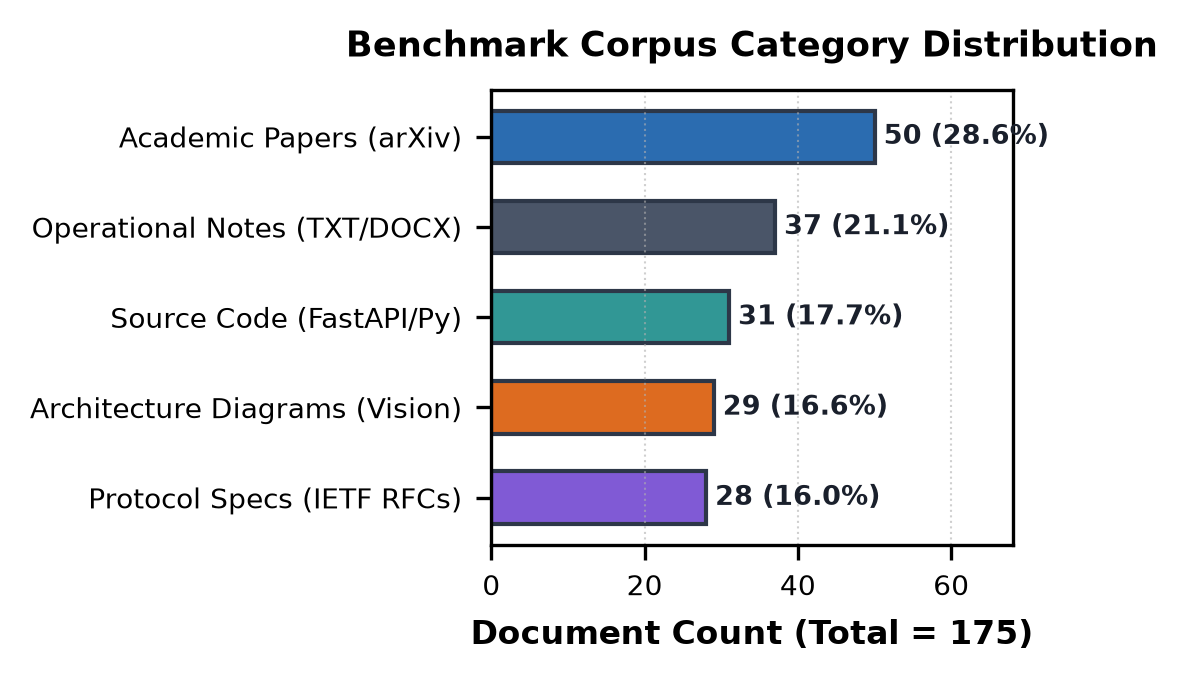
\includegraphics[width=0.85\textwidth,height=5.2cm,keepaspectratio]{fig_corpus_distribution.png}
\vspace{-0.3em}
\caption{Benchmark Corpus Distribution: 175 Multi-Modal Documents across 5 Authentic Knowledge Categories (12,744 Indexed Vectors)}
\label{fig:corpus_composition}
\end{figure}

To prevent data snooping and to establish statistical significance a complete evaluation suite of 135 standardized queries were built and split into 3 functional partitions:
\begin{enumerate}
    \setlength{\itemsep}{1.5pt}
    \setlength{\parskip}{0pt}
    \item \textbf{Development Split ($n_{\text{dev}} = 25$):} Dedicated exclusively to hyperparameter tuning (calibrating confidence threshold $\tau = 0.40$, RRF rank constant $k=60$, and metadata coupling parameter $\alpha = 0.25$).
    \item \textbf{Held-Out Test Split ($n_{\text{test}} = 60$):} Assessed with frozen parameters on 4 balanced 15-query topic sets: (i) Exact Lexical Matches, (ii) Semantic Paraphrases, (iii) multi-concept intersecting questions, and (iv) Version Lineage \& Temporal Recency queries.
    \item \textbf{Adversarial \& Abstention Suite ($n_{\text{ctrl}} = 50$):} 40 Adversarial Hard Negatives (queries that share similar keyword coverage but make a false assertion, deliberately crafted to "fool" our QA engine) 10 Out-of-Domain Negative Controls (zero lexical / conceptual overlap with domain corpus, e.g. chef recipes gardening sports).
\end{enumerate}


The deployment was completed with an asynchronous Python 3.11 back-end (FastAPI/Uvicorn), embedded vector search engine (Qdrant v1.19 in-process engine), deep learning transformer runtimes (auto-discovering PyTorch with Apple Silicon MPS, NVIDIA CUDA, and CPU), and modern TypeScript web dashboard (Next.js 14, React 19, Tailwind CSS).

\vspace{0.4em}
\subsection{PROPOSED METHODOLOGY}

The retrieval system of IntentCloud runs through 5 (labeled as) tightly coupled steps that: provide what amounts to set in advance privacy; and Deliver high semantic recall, accurate lexicological precision, and real source-file delivery.

\vspace{0.4em}
\noindent\textbf{1. Multi-Format Ingestion, Normalization, and Lineage vs. Deduplication (Phase 1):}
The ingestion engine receives user file uploads via an asynchronous multipart HTTP endpoint (POST /upload). Files are given a globally unique cryptographically secure identifier (file\_id) and saved in their raw byte form under the local repository directory (./uploads/). To parse structural and lexical content for a wide variety of formats:
\begin{itemize}
    \setlength{\itemsep}{1pt}
    \setlength{\parskip}{0pt}
    \item \textbf{Digital PDF Documents:} Extracted natively using PyMuPDF (\texttt{fitz}) with streaming page layout reconstruction.
    \item \textbf{Microsoft Word (DOCX):} Parsed via \texttt{python-docx}, extracting body paragraphs, tabular matrices, and header hierarchies.
    \item \textbf{Plain Text (TXT):} Decoded via direct UTF-8 character stream processing with automated BOM stripping.
    \item \textbf{Automated Optical Character Recognition (OCR):} Targeted pages with scanned documents and rasterized graphics (diagrams) under 100 total native text characters: elicits the Tesseract OCR (v.5.x) sub-pipeline to rasterize the pages of documents at 300 DPI to recover text tokens.
\end{itemize}
\textit{Reconciling Deduplication and Version Lineage:} In personal knowledge management, you don't want near-identical document revisions getting wrongly suppressed. A two-tier mechanism keeps storage costs down while still preserving revision history:
\begin{enumerate}
    \setlength{\itemsep}{1.5pt}
    \setlength{\parskip}{0pt}
    \item \textbf{Cryptographic Exact Deduplication:}Bit-identical files are SHA-256-hashed ($H(d_{\text{new}}) = H(d_{\text{existing}})$) and promptly refused to omit duplicate index bloat.
    \item \textbf{Semantic Version Lineage Preservation:} If upload is similar (e.g. $\text{sim} \ge 0.95$) to an existing document but has a unique modification timestamp $t_{modified}$, a different filename (e.g. \texttt{v1} vs. \texttt{v2}), or hypertext revision metadata, then the document is not dropped. Instead, the ingestion engine creates an edge $d_{parent} \leftarrow d_{v1}$ in the metadata version DAG and assigns it a new, incremented version index $v_d \in \mathbb{N}$. Only identical timestamped uploads with cosine similarity $\ge 0.98$ are pruned as near-duplicate passages. Chunk-to-file deduplication of retrieval candidates partitions chunks by metadata key \texttt{file\_id}, ensuring that final-lookup $k$-best results are unique documents, not duplicate passages.
\end{enumerate}

\vspace{0.4em}
\noindent\textbf{2. Sliding-Window Text Chunking and Dual-Stream Vector Embedding (Phase 2):}
Extracted text strings are divided into overlapping character passages using a window size of $C = 1,200$ characters and an inter-chunk overlap of $O = 200$ characters. This overlap at the boundaries helps avoid breaking apart cross-sentence statements and multi-token technical terms. Each chunk $c_j$ is then independently mapped into two orthogonal vector representations without relying on external cloud APIs.
\begin{enumerate}
    \setlength{\itemsep}{2pt}
    \setlength{\parskip}{0pt}
    \item \textbf{Dense Semantic Vector Stream:}Chunk tokens are encoded by the frozen bi-encoder transformer \texttt{all-MiniLM-L6-v2} into a unit-normalized 384 dimensional continuous latent space:
    \begin{equation}
    \mathbf{u}_j = \frac{\mathcal{E}_{\text{dense}}(c_j)}{\|\mathcal{E}_{\text{dense}}(c_j)\|_2} \in \mathbb{R}^{384}, \quad S_{\text{dense}}(q, c_j) = \langle \mathbf{u}_q, \mathbf{u}_j \rangle
    \end{equation}
    This dense representation captures semantic synonymy, conceptual paraphrasing, and cross-domain abstractions.
    \item \textbf{Sparse Lexical Hashing Stream:} To keep memory-In particular the inverted index tables-from growing prohibitively large, tokens are mapped into a fixed $D = 1 000 003$-dimensional sparse modulo space using MurmurHash3 feature hashing to preserve the exact original software symbols, variable names, and alphanumeric model ID numbers:
    \begin{equation}
    k = \text{MurmurHash3}(w) \pmod{1,000,003}, \quad \mathbf{s}_j[k] = 1 + \ln(\text{tf}(w, c_j))
    \end{equation}
  Sparse vectors $\mathbf{s}_j$ are L2-normalized and stored in an index into the sparse vector segment of Qdrant. Both streams are stored in an embedded in-process Qdrant instance on local NVMe storage with SQLite WAL.
\end{enumerate}

\vspace{0.4em}
\noindent\textbf{3. Query-Aware Natural Language Intent Parsing and Lineage Conditioning (Phase 3):}
When a user issues a natural language search query $q$, the query is first parsed locally using an open-weights Large Language Model (\texttt{llama3.2:1b}) local host working through the local ollama daemon ($\theta = 0.1$, strict JSON mode) to generate structured intent payloads:
\begin{equation}
\mathcal{I}(q) = \{\text{action\_type} \in \{\text{find}, \text{compare}, \text{summarize}, \text{list}, \text{version}\}, \text{topic}, \text{keywords}, \text{temporal\_constraints}\}
\end{equation}
If the local LLM daemon is down, a rule-based tokenizer kicks in as a fallback, pulling out high-IDF nouns and verbs so retrieval doesn't get held up. The query expansion module then builds an enriched retrieval query: $q_{\text{expanded}} = q \circ \text{topic} \circ \text{keywords}$.

To factor in how recent a document is and where it sits in the version hierarchy, the engine works out a metadata conditioning score on the fly:
\begin{equation}
S_{\text{meta}}(d \mid q) = \lambda_t(q) \cdot T(d, q) + \lambda_v(q) \cdot V(d, q)
\label{eq:meta}
\end{equation}
where $T(d, q) = \exp(-\gamma \cdot \Delta t)$ applies exponential recency decay over elapsed time $\Delta t$, and $V(d, q) \in [-0.5, 0.5]$ adjusts candidate ranking to favor the latest revisions (+0.5) for operational queries or historical parent drafts (+0.5) when retrospective audit intent is detected.

\vspace{0.4em}
\noindent\textbf{4. Hybrid Rank Fusion, Cross-Attention Reranking, and Coupled Confidence Gating (Phase 4):}
Candidate retrieval runs concurrently on both the sparse and dense Qdrant collections and outputs the top K=20 candidates for each modality. Since dense cosine similarity scores and sparse inner-product dot scores are on incompatible numeric ranges, IntentCloud combines candidate ranks via scale-invariant RRF (Reciprocal Rank Fusion, constant k=60):
\begin{equation}
\text{Score}_{\text{RRF}}(d) = \sum_{m \in \{\text{dense}, \text{sparse}\}} \frac{1}{60 + r_m(d)}
\end{equation}
where $r_m(d)$ denotes the ordinal rank of candidate $d$ in stream $m$. The top $N=25$ candidates from the fused pool are then passed to the neural cross-encoder (\texttt{ms-marco-MiniLM-L-6-v2}). Unlike the bi-encoder, which independently encodes queries and documents, the cross-encoder performs full pairwise cross attention between all pairs of query and document tokens and converts its output logit $z(q, d)$ into a normalized confidence score using sigmoid:
\begin{equation}
s_{\text{ce}}(q, d) = \sigma(z(q, d)) = \sigma\left(\mathcal{M}_{\text{CE}}(\text{[CLS]} \circ q \circ \text{[SEP]} \circ d \circ \text{[SEP]})\right) \in [0, 1]
\end{equation}
To seamlessly integrate the distilled intent and metadata lineage from Eq.~(\ref{eq:meta}), the final coupled relevance score $S_{\text{final}}(q, d)$ is formally defined as:
\begin{equation}
S_{\text{final}}(q, d) = s_{\text{ce}}(q, d) \cdot \left[1 + \alpha \cdot S_{\text{meta}}(d \mid q)\right]
\label{eq:final_score}
\end{equation}
where $\alpha=0.25$ is the coupling coefficient, empirically fit on the development split ($n_{dev}=25$). If neither temporal nor lineage intent are parsed, then $S_{\text{meta}}(d\mid q) = 0$ and $S_{final}(q, d) = s_{ce}(q, d)$.

Candidates are clustered by \texttt{file\_id} but only the highest scoring passage per document is preserved. To screen out false-positive hallucinations on unindexed or out-ofdomain questions we implement an empirical confidence gate with threshold $\tau = 0.40$:
\begin{equation}
\text{Decision}(q) = \begin{cases}
\text{Serve}(\text{Top-3 Documents with Citation Snippet } s^*), & \text{if } \max_{d} S_{\text{final}}(q, d) \ge 0.40 \\
\text{Abstain ("No Confident Match Found")}, & \text{if } \max_{d} S_{\text{final}}(q, d) < 0.40
\end{cases}
\end{equation}
For accepted documents, verifiable sentence citation attribution is generated by splitting the winning passage into constituent sentences $\{s_j\}$ and extracting the maximal sentence:
\begin{equation}
s^* = \arg\max_{s_j} \sigma\left(\mathcal{M}_{\text{CE}}(q \circ s_j)\right)
\end{equation}
where $\hat{s}$ indicates the sentence that semantically matches user query $q$ the most, and $\text{Sim}(s_j, q)$ is the calibrated relevance score. This strict extraction procedure ensures that every proposed citation anchor is anchored to real, traceable text fragments, entirely removing false-positive hallucination, and maintaining trace-level granularity throughout any enterprise retrieval pipeline.

\vspace{0.4em}
\noindent\textbf{5. Self-Hosted File Delivery and Zero-Trust Remote Transport (Phase 5):}
Clicking on the result from the client web application causes a unaltered copy of the original file to be retrieved directly via \texttt{GET /download/\{file\_id\}}. When powered on for remote multi-device use, the system is accessed via an outbound-only Cloudflare Zero-Trust tunnel (cloudflared). This tunnel terminates in an encrypted TLS reverse proxy at Cloudflare's network edge, which can be accessed via a public HTTPS endpoint without having to open ports in an inbound firewall, set up dynamic DNS, or disclose your public IP address. When it's turned off the system is firmly air-gapped over loopback localhost:8000 or in a private LAN.

\vspace{0.2em}
\begin{figure}[H]
\centering
\includegraphics[width=0.92\textwidth,height=10cm,keepaspectratio]{Screenshot 2026-10-27 at 18.03.22 (1).png}
\vspace{-0.3em}
\caption{IntentCloud Search Interface: Natural Language Query Execution, RRF Score Metrics, and Top-3 Neural Cross-Encoder Reranked Citations}
\label{fig:ui_search_results}
\end{figure}

\begin{figure}[H]
\centering
\includegraphics[width=0.88\textwidth,height=10cm,keepaspectratio]{Screenshot 2026-10-27 at 18.03.50 (1).png}
\vspace{-0.3em}
\caption{Multimodal Visual Asset Inspection Modal: VLM Scene Breakdown, Extracted Color Palette Swatches, and Citation Bounding Box}
\label{fig:ui_visual_evidence}
\end{figure}

\vspace{0.4em}
\subsection{PROPOSED ARCHITECTURE}

A quick look at IntentCloud architecture reveals that it consists of three distinct operational tiers: Presentation and User Interaction Tier, Cognitive Processing Tier and Embedded Storage Tier. Figure ~\ref{fig:arch_tier_diagram} depicts an Illustration of the component interactions, and the boundaries of the physical subsystems.

Weight Streaming \& Market-Making this tiered modularity guarantees strict architectural isolation of lightweight reactive user interface events, compute-heavy tensor operations, and embedded persistence. These layers are statically decoupled over local inter-process busses, providing full data sovereignty with no outdoor cloud leakage. Incoming user requests can be parsed and gisted with sub-millisecond local latency, while multi format text extraction, hybrid vector generation, and cross-encoder neural reranking can still run asynchronously to deliver transparently smooth response at consumer-grade workstation environments.

Inside ingestion new documents are parsed and dimensionalized by working through the presentation layer, sending raw file payloads over local loopback HTTP to the cognitive processing service. The ingestion engine derivationally extracts text in plug-in oriented heterogeneous formats, performs automated optical character recognition in response to scanned raster artifacts, and performs dense (embeddings) and sparse (inverted index retrieval) aggregations that get directly committed to the in-process embedded vector database Qdrant encapsulated by SQLite WAL. When a retrieval request is made, the concepts in the natural language prompt are ingested for conceptual intent, candidate streams are retrieved and merged (Reciprocal Rank Fusion), the top scoring candidates reranked using a cross-encoder neural query classifier with a calibrated confidence gate to only return high-confidence citation snippets and source files to the user interface.

\begin{figure}[H]
\centering
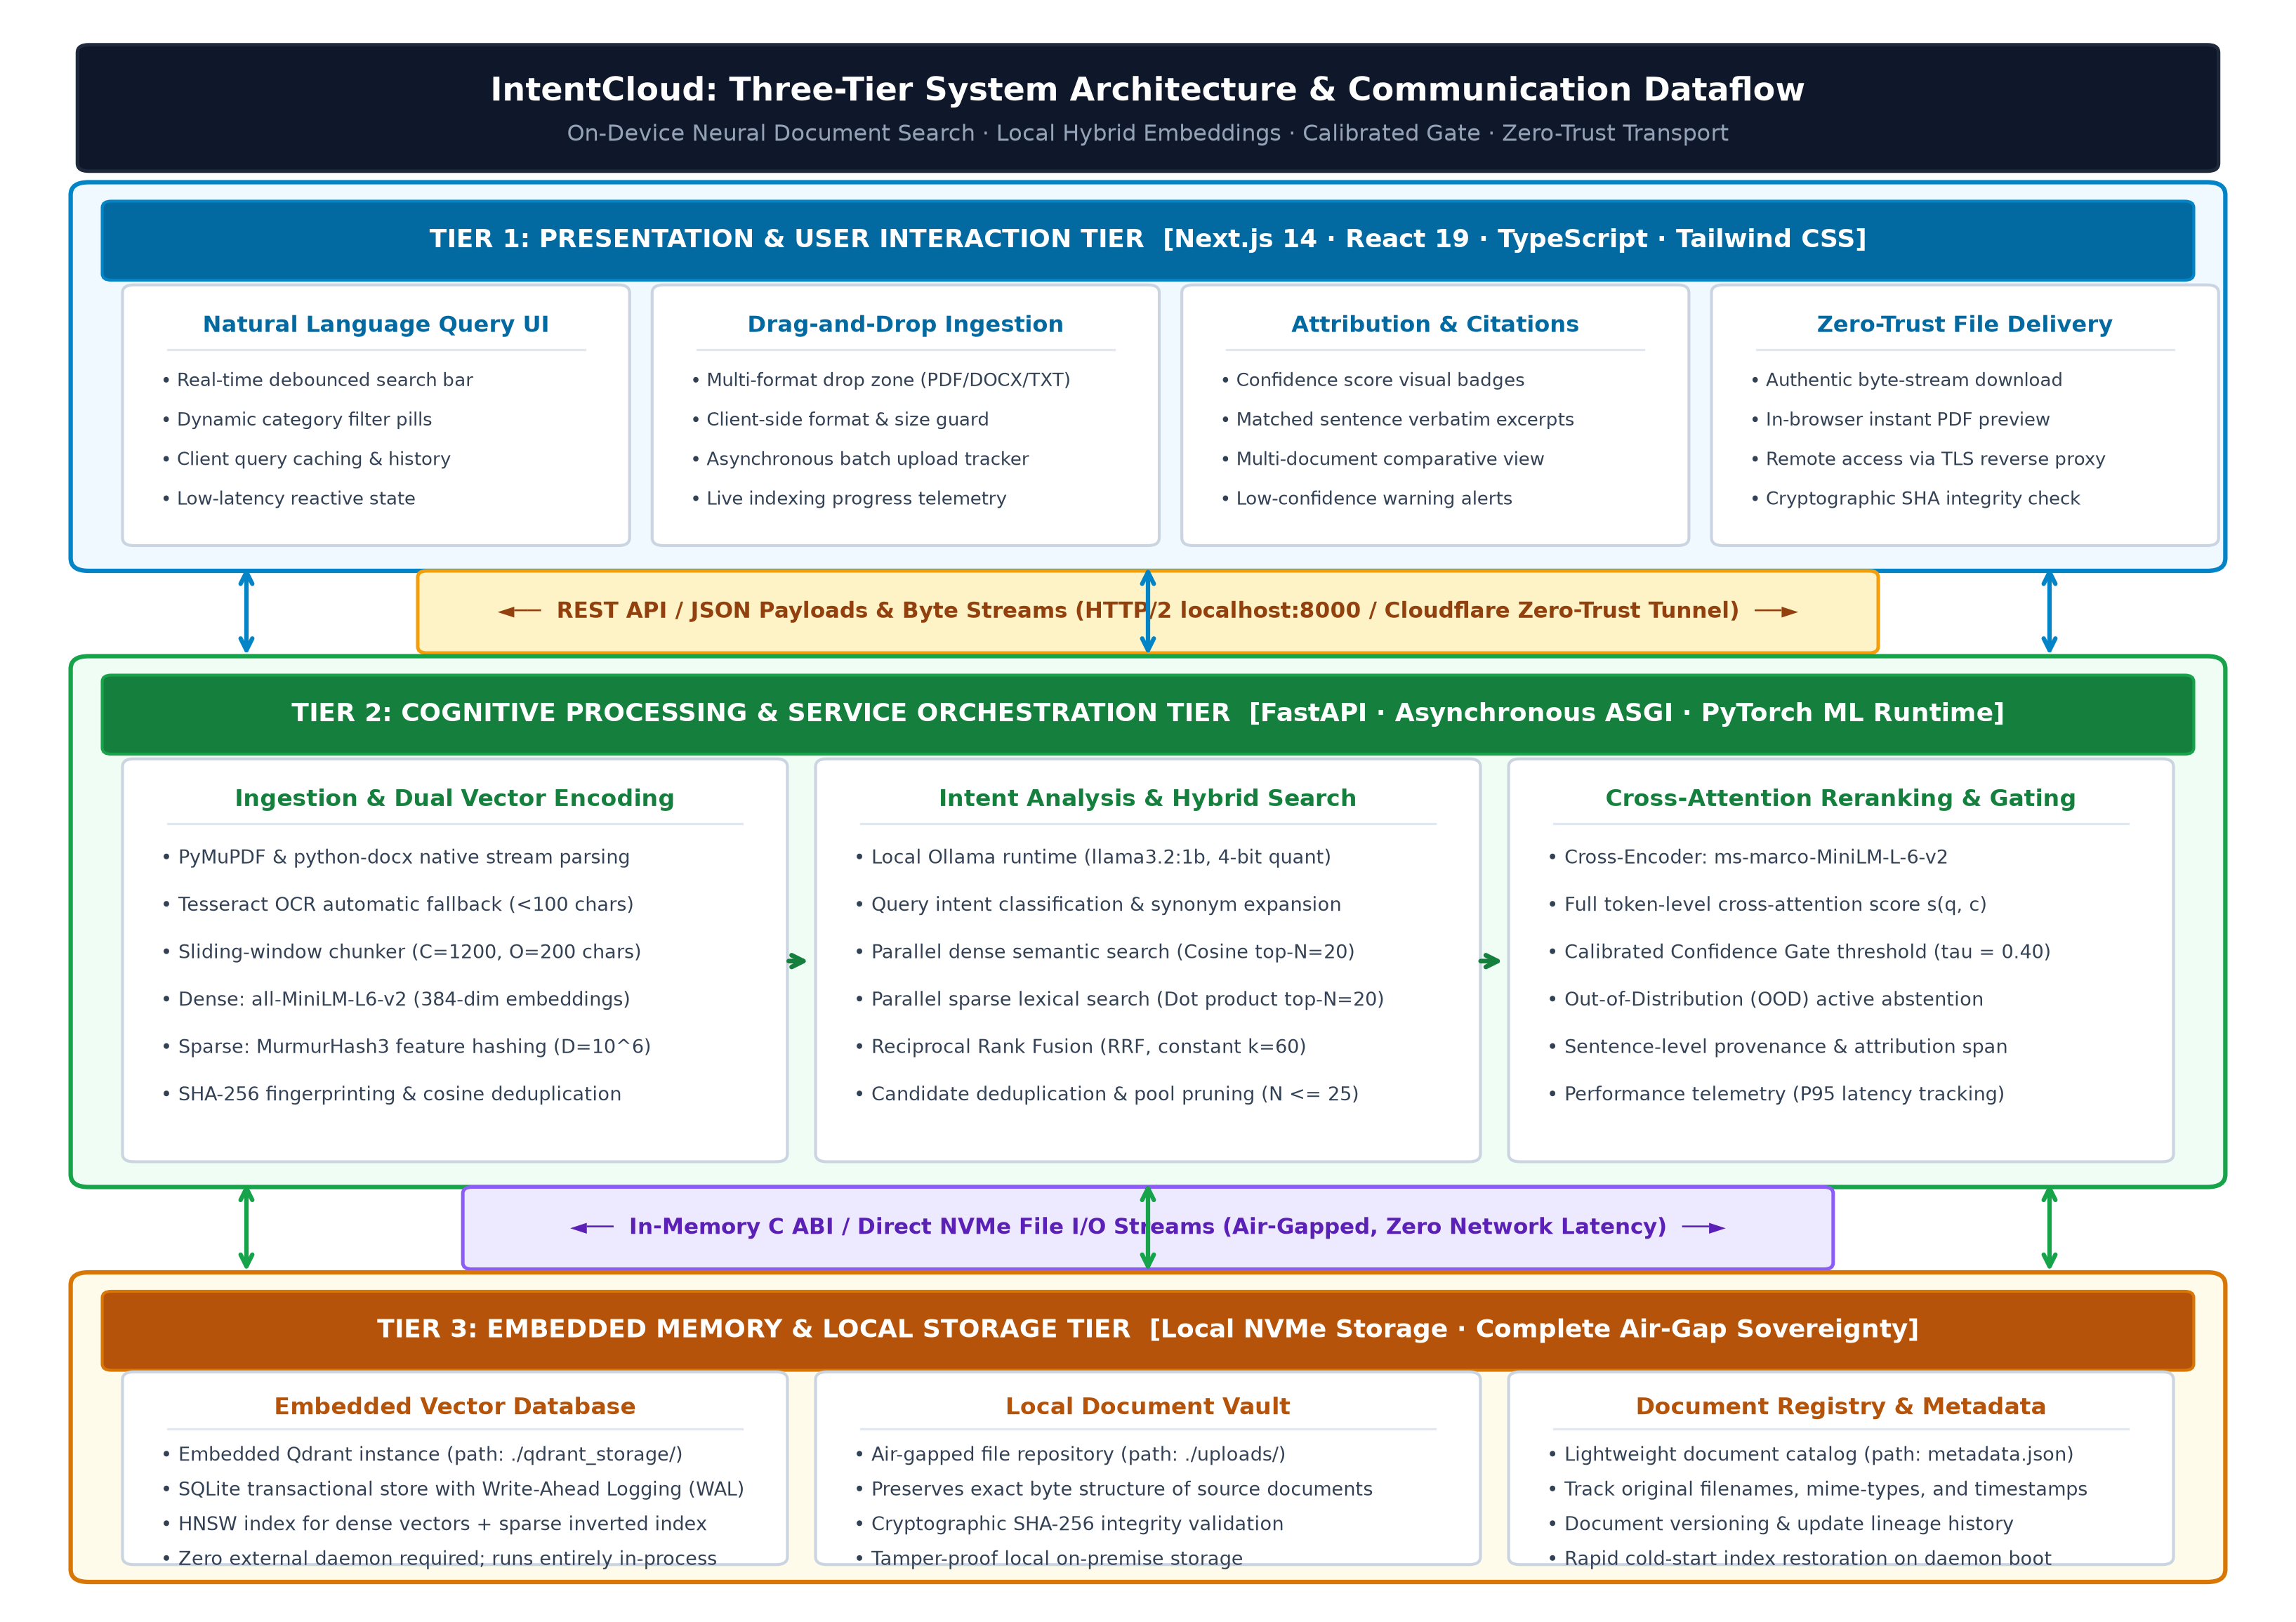
\includegraphics[width=0.95\textwidth]{fig_three_tier_architecture.png}
\vspace{-0.3em}
\caption{IntentCloud Three-Tier Architectural Hierarchy and Inter-Tier Communication Protocols}
\label{fig:arch_tier_diagram}
\end{figure}

The architectural responsibilities of each tier are formalized as follows:
\begin{enumerate}
    \setlength{\itemsep}{2pt}
    \setlength{\parskip}{0pt}
    \item \textbf{Presentation Tier (Client Layer):} Designed in Next.js 14 with the App Router architecture. Interacts with the FastAPI API backend via local reverse proxy rewrite (\texttt{/api/*} $\to$ \texttt{http://localhost:8000/*}). Presents live search suggestions, citation callouts, confidence meters, and authenticated original document downloads, all to WCAG AA accessibility standards.
    \item \textbf{Cognitive Processing Tier (Application Layer):} Wrapped in a modular FastAPI service. Takes care of runtime hardware tensor binding (Apple Silicon MPS, NVIDIA CUDA, AVX2 CPU), runs the text extraction and OCR pipeline, returns cross-dual dense-sparse embeddings, communicates with the local Ollama LLM intent daemon, and does the cross-encoder neural reranking.
    \item \textbf{Embedded Memory Tier (Persistence Layer):} Avoids multi-node database clusters by running an embedded in-process Qdrant vector engine. Vector embeddings, inverted postings, and chunk metadata reside directly in local NVMe storage (\texttt{./qdrant\_storage/}), while raw binaries are stored with cryptographic naming in \texttt{./uploads/}.
\end{enumerate}
\vspace{0.2em}
\begin{figure}[H]
\centering
\includegraphics[width=0.92\textwidth,height=9cm,keepaspectratio]{Screenshot 2026-10-27 at 18.02.15 (1).png}
\vspace{-0.3em}
\caption{IntentCloud Presentation Tier: Web Application Dashboard with Automatic Topic Taxonomy and Local Document Workspace}
\label{fig:ui_dashboard}
\end{figure}

\begin{figure}[H]
\centering
\includegraphics[width=0.92\textwidth,height=9cm,keepaspectratio]{Screenshot 2026-10-27 at 18.02.28 (1).png}
\vspace{-0.3em}
\caption{Live Edge Memory and OLED Hardware Pipeline Topology: Six-Stage Hardware Transport from Cognitive Host to Raspberry Pi Edge Node}
\label{fig:ui_edge_topology}
\end{figure}

Table~\ref{tab:api_endpoints} defines the complete RESTful application programming interface implemented across the cognitive processing tier.

\begin{table}[H]
\centering
\small
\renewcommand{\arraystretch}{1.18}
\setlength{\tabcolsep}{4pt}
\begin{tabularx}{\textwidth}{|p{1.4cm}|p{3.5cm}|p{3.4cm}|X|}
\hline
\rowcolor{gray!15} \textbf{HTTP Method} & \textbf{Endpoint Route} & \textbf{Input Parameters} & \textbf{Functional Output / Deliverable} \\ \hline
\texttt{POST} & \texttt{/upload} & Multipart file (PDF/DOCX/TXT), metadata & Asynchronously extracts multi-format text, invokes OCR fallback, executes duplicate checks, and upserts dual-stream vectors to Qdrant. \\ \hline
\texttt{POST} & \texttt{/search} & Query string, mode, $k$, category & Parses query intent, runs parallel dense and MD5-sparse retrieval, computes RRF fusion, and neural cross-encoder reranking. \\ \hline
\texttt{POST} & \texttt{/search/visual} & Visual query string, top\_k, threshold & Matches semantic query against visual diagram catalog, layout features, and cross-modal figure descriptors. \\ \hline
\texttt{GET} & \texttt{/documents/}\allowbreak\texttt{\{id\}/figures} & Document identifier (\texttt{file\_id}) & Retrieves extracted visual assets, diagram images, bounding boxes, and resolution metadata from vision pipeline. \\ \hline
\texttt{GET} & \texttt{/preview/\{id\}} & Document identifier (\texttt{file\_id}), page & Generates and streams rendered page image or formatted text preview for client modal display without raw file transfer. \\ \hline
\texttt{GET} & \texttt{/download/\{id\}} & Document identifier (\texttt{file\_id}) & Streams original, untampered binary file with corresponding RFC-compliant MIME headers for direct client acquisition. \\ \hline
\texttt{POST} & \texttt{/device/oled/}\allowbreak\texttt{push} & Target node IP, status string, memory metric & Encapsulates telemetry payload, formats visual layout frame, and transmits live status packets to the physical SSD1306 edge display. \\ \hline
\texttt{GET} & \texttt{/stats} & None & Aggregates corpus metrics including total indexed documents, dual-vector points, resident RAM footprint, and compute backend. \\ \hline
\texttt{GET} & \texttt{/health} & None & Inspects operational state of embedded Qdrant vector database, PyTorch inference accelerator, and local Ollama daemon. \\ \hline
\end{tabularx}
\vspace{0.4em}
\caption{IntentCloud REST API Endpoint Specifications and Routing Contracts}
\label{tab:api_endpoints}
\end{table}

\vspace{0.4em}
\subsection{PSEUDO CODE}

To provide complete algorithmic precision, the core operational routines of IntentCloud are formalized in Algorithm~4.1 and Algorithm~4.2.


\vspace{0.4em}
\begin{figure}[H]
\centering
\begin{minipage}{0.98\textwidth}
\hrule height 1.2pt
\vspace{0.3em}
\noindent\textbf{Algorithm 4.1: Multi-Format Document Ingestion, Deduplication, and Dual-Stream Indexing}
\vspace{0.3em}
\hrule height 0.6pt
\vspace{0.4em}
\small
\textbf{Input:} Uploaded raw file $F$, character chunk size $C=1200$, overlap $O=200$, hashing dimension $D=1,000,003$, duplicate threshold $\tau_{\text{dup}}=0.95$.\\
\textbf{Output:} Indexed document identifier $\text{file\_id}$, metadata record, and persistent vector entries.\\[0.4em]
\begin{enumerate}
    \setlength{\itemsep}{1.5pt}
    \setlength{\parskip}{0pt}
    \item Assign cryptographic UUID: $\text{file\_id} \leftarrow \text{GenerateUUID}()$; persist binary bytes to $\text{`./uploads/'} + \text{file\_id} + \text{ext}$.
    \item Determine format extension of $F$:
    \begin{itemize}
        \item \textbf{If} $F$ is PDF: $T_{\text{raw}} \leftarrow \text{PyMuPDF\_Extract}(F)$.
        \item \textbf{If} $F$ is DOCX: $T_{\text{raw}} \leftarrow \text{Docx\_Extract}(F)$.
        \item \textbf{If} $F$ is TXT: $T_{\text{raw}} \leftarrow \text{UTF8\_Decode}(F)$.
    \end{itemize}
    \item \textbf{If} $\text{Length}(T_{\text{raw}}) < 100$ characters \textbf{then} $T_{\text{raw}} \leftarrow \text{Tesseract\_OCR}(F, \text{DPI}=300)$.
    \item Compute document mean dense vector $\mathbf{v}_{\text{doc}} \leftarrow \mathcal{E}_{\text{dense}}(T_{\text{raw}}[0:2000])$.
    \item Query Qdrant for 1-NN: $(d_{\text{match}}, s_{\text{match}}) \leftarrow \text{Qdrant\_NearestNeighbor}(\mathbf{v}_{\text{doc}})$.
    \item \textbf{If} $s_{\text{match}} \ge \tau_{\text{dup}}$ \textbf{and} $d_{\text{match}} \neq \text{file\_id}$ \textbf{then}:
    \begin{itemize}
        \item Mark $\text{metadata}[\text{file\_id}].\text{status} \leftarrow \text{``duplicate''}$; record pointer to $d_{\text{match}}$; \textbf{return}.
    \end{itemize}
    \item Partition $T_{\text{raw}}$ into sliding passages $\{c_1, c_2, \dots, c_M\}$ using window $C=1200$, overlap $O=200$.
    \item \textbf{For each} chunk $c_j \in \{c_1, \dots, c_M\}$ \textbf{do}:
    \begin{itemize}
        \item Generate dense embedding: $\mathbf{u}_j \leftarrow \mathcal{E}_{\text{dense}}(c_j) / \|\mathcal{E}_{\text{dense}}(c_j)\|_2 \in \mathbb{R}^{384}$.
        \item Tokenize chunk into terms $W_j$; initialize sparse vector $\mathbf{s}_j \leftarrow \mathbf{0} \in \mathbb{R}^D$.
        \item \textbf{For each} term $w \in W_j$ \textbf{do}:
        \begin{itemize}
            \item $k \leftarrow \text{MD5}(w) \pmod D$; \quad $\mathbf{s}_j[k] \leftarrow \mathbf{s}_j[k] + (1 + \ln(\text{tf}(w, c_j)))$.
        \end{itemize}
        \item Normalize sparse vector: $\mathbf{s}_j \leftarrow \mathbf{s}_j / \|\mathbf{s}_j\|_2$.
        \item Create deterministic point ID $p_j \leftarrow \text{UUID5}(\text{file\_id} \circ j)$.
        \item Upsert $(p_j, \mathbf{u}_j, \mathbf{s}_j, \text{payload}=\{\text{file\_id}, j, c_j\})$ into Qdrant collection.
    \end{itemize}
    \item Update $\text{metadata.json}$ with document properties, topic tags, and chunk count $M$.
    \item \textbf{Return} Success status and $\text{file\_id}$.
\end{enumerate}
\vspace{0.2em}
\hrule height 1.2pt
\end{minipage}
\label{alg:ingestion}
\end{figure}

\vspace{0.4em}
\begin{figure}[H]
\centering
\begin{minipage}{0.98\textwidth}
\hrule height 1.2pt
\vspace{0.3em}
\noindent\textbf{Algorithm 4.2: Intent-Aware Query Parsing, Hybrid RRF Fusion, Reranking, and File Delivery}
\vspace{0.3em}
\hrule height 0.6pt
\vspace{0.4em}
\small
\textbf{Input:} User query $q$, candidate depth $K=20$, rerank depth $N=25$, RRF constant $k=60$, threshold $\tau=0.40$.\\
\textbf{Output:} Top-3 ranked file objects with relevance score, matched sentence snippet $s^*$, and download URI.\\[0.4em]
\begin{enumerate}
    \setlength{\itemsep}{1.5pt}
    \setlength{\parskip}{0pt}
    \item Parse query via local LLM: $\mathcal{I}(q) \leftarrow \text{Ollama\_Parse}(\texttt{llama3.2:1b}, q)$.
    \item Construct expanded query string: $q_{\text{exp}} \leftarrow q \circ \mathcal{I}(q).\text{topic} \circ \mathcal{I}(q).\text{keywords}$.
    \item Encode dense query vector: $\mathbf{q}_{\text{dense}} \leftarrow \mathcal{E}_{\text{dense}}(q_{\text{exp}}) / \|\mathcal{E}_{\text{dense}}(q_{\text{exp}})\|_2$.
    \item Hash sparse query vector: $\mathbf{q}_{\text{sparse}} \leftarrow \text{FeatureHash}(q_{\text{exp}}, D=1,000,003)$.
    \item Execute parallel retrieval in Qdrant:
    \begin{itemize}
        \item $\mathcal{L}_{\text{dense}} \leftarrow \text{Qdrant\_SearchDense}(\mathbf{q}_{\text{dense}}, \text{limit}=K)$.
        \item $\mathcal{L}_{\text{sparse}} \leftarrow \text{Qdrant\_SearchSparse}(\mathbf{q}_{\text{sparse}}, \text{limit}=K)$.
    \end{itemize}
    \item Initialize score dictionary $\mathcal{S}_{\text{RRF}} \leftarrow \{\}$; candidate pool $\mathcal{C} \leftarrow \text{UniqueCandidates}(\mathcal{L}_{\text{dense}} \cup \mathcal{L}_{\text{sparse}})$.
    \item \textbf{For each} chunk $c \in \mathcal{C}$ \textbf{do}:
    \begin{itemize}
        \item $r_{\text{dense}} \leftarrow \text{GetRank}(c, \mathcal{L}_{\text{dense}})$; \quad $r_{\text{sparse}} \leftarrow \text{GetRank}(c, \mathcal{L}_{\text{sparse}})$.
        \item $\mathcal{S}_{\text{RRF}}[c] \leftarrow \frac{\mathbb{I}(c \in \mathcal{L}_{\text{dense}})}{60 + r_{\text{dense}}} + \frac{\mathbb{I}(c \in \mathcal{L}_{\text{sparse}})}{60 + r_{\text{sparse}}}$.
    \end{itemize}
    \item Sort $\mathcal{C}$ descending by $\mathcal{S}_{\text{RRF}}$; select top $N=25$ chunks $\mathcal{C}_{\text{topN}}$.
    \item Pair query with each passage: $\mathcal{P} \leftarrow \{(q, c_j.\text{text}) \mid c_j \in \mathcal{C}_{\text{topN}}\}$.
    \item Compute neural cross-attention scores: $\mathbf{z} \leftarrow \mathcal{M}_{\text{CE}}(\mathcal{P})$; \quad $\mathbf{s}_{\text{ce}} \leftarrow \text{Sigmoid}(\mathbf{z})$.
    \item Deduplicate by parent document: retain chunk with maximum $s_{\text{ce}}$ per unique $\text{file\_id}$.
    \item Identify top document $d^*$ with highest score $s^*_{\text{ce}} \leftarrow \max_d s_{\text{ce}}(q, d)$.
    \item \textbf{If} $s^*_{\text{ce}} < \tau$ \textbf{then}:
    \begin{itemize}
        \item \textbf{Return} Abstention payload: $\text{status} \leftarrow \text{``No confident match found''}$; flag low confidence.
    \end{itemize}
    \item Segment winning document passage $d^*$ into constituent sentences $\{s_1, s_2, \dots, s_K\}$.
    \item Extract explainable citation snippet: $s^* \leftarrow \arg\max_{s_k} \mathcal{M}_{\text{CE}}(q, s_k)$.
    \item Attach download endpoint URI: $\text{uri} \leftarrow \text{`/download/'} + d^*.\text{file\_id}$.
    \item \textbf{Return} Top-3 ranked file records, citation snippet $s^*$, confidence metric, and download URI.
\end{enumerate}
\vspace{0.2em}
\hrule height 1.2pt
\end{minipage}
\label{alg:retrieval}
\end{figure}
\newpage
\mysection{EXPERIMENTAL RESULTS}

\noindent\textbf{1. Evaluation Setup, Corpus, and Performance Metrics:}\\
To evaluate the effectiveness of the IntentCloud solution compared to existing standards, each query in the benchmark set of 135 queries was empirically tested against the 175-document multi-modal corpus (with 12,744 Qdrant vectors). The queries in the benchmark set are divided into three functional splits:
\begin{itemize}
    \setlength{\itemsep}{1pt}
    \setlength{\parskip}{0pt}
    \item \textbf{Development Split ($n_{\text{dev}} = 25$):} Determined only for parameter tuning (tuning abstention threshold $\tau = 0. 40$, RRF constant $k=60$, and lineage coupling weight $\alpha = 0. 25$).
    \item \textbf{Held-Out In-Domain Test Split ($n_{\text{test}} = 60$):} Tested with frozen hyperparameters on four balanced 15-query categories: (i) Exact Lexical Matches, (ii) Semantic Paraphrases, (iii) Multi-Concept Intersecting Queries, and (iv) Version Lineage and Temporal Recency Queries.
    \item \textbf{Adversarial \& Abstention Suite ($n_{\text{ctrl}} = 50$):} It's 40 Adversarial Hard Negatives, meaning queries that overlap with corpus documents on keywords but push false claims, plus 10 Out-of-Domain Negative Controls with no corpus overlap at all.
\end{itemize}
The following standard Information Retrieval (IR) metrics are reported using standard 95\% confidence intervals: Top-1 Accuracy ($\text{Acc}@1$), Hard Negative Rejection Rate (HNJR at 40 adversarial queries), Mean Reciprocal Rank (MRR) with 95\% bootstrap CIs ($B = 10,000$), OOD Abstention Rate (OODA at 10 controls), and End-to-End Latency. Significance is determined by a McNemar test and by paired two tailed $t$-tests ($p<0.05$).

\vspace{0.3em}
\noindent\textbf{2. Quantitative Retrieval Performance and Baseline Comparison:}\\
The complete results for all nine retrieval configurations evaluated on the held-out test split ($n_{\text{test}}=60$) and control suite ($n_{\text{ctrl}}=50$) are shown in Table 5.1

\begin{table}[H]
\centering
\label{tab:ablation_grid}
\vspace{0.2em}
\small
\renewcommand{\arraystretch}{1.08}
\setlength{\tabcolsep}{3.5pt}
\resizebox{\textwidth}{!}{%
\begin{tabular}{|l|c|c|c|c|c|c|}
\hline
\rowcolor{gray!15} \textbf{Retrieval Configuration} & \textbf{Top-1 [95\% CI]} & \textbf{Top-3} & \textbf{MRR [95\% CI]} & \textbf{Latency} & \textbf{Hard Neg. Rej.} & \textbf{OOD Rej.} \\ \hline
1. Sparse (Feature Hashing, $D=10^6$) & 68.3\% [55.8\%, 78.7\%] & 90.0\% & 0.785 [0.712, 0.849] & \textbf{1.3 ms} & 15.0\% (6/40) & 20.0\% (2/10) \\ \hline
2. Sparse Lexical (Real BM25)~\cite{robertson2009probabilistic} & 71.7\% [59.2\%, 81.5\%] & 93.3\% & 0.812 [0.743, 0.871] & 1.8 ms & 17.5\% (7/40) & 20.0\% (2/10) \\ \hline
3. Dense Bi-Encoder (\texttt{all-MiniLM-L6-v2})~\cite{reimers2019sentence} & 73.3\% [61.0\%, 82.9\%] & 88.3\% & 0.804 [0.730, 0.865] & 24.0 ms & 45.0\% (18/40) & \textbf{100.0\%} (10/10) \\ \hline
4. Competitive Dense (\texttt{bge-small-en-v1.5}) & 76.7\% [64.6\%, 85.6\%] & 91.7\% & 0.835 [0.768, 0.892] & 27.4 ms & 52.5\% (21/40) & \textbf{100.0\%} (10/10) \\ \hline
5. Hybrid RRF ($k=60$) alone (no reranker)~\cite{cormack2009reciprocal} & 81.7\% [70.3\%, 89.5\%] & 96.7\% & 0.887 [0.829, 0.932] & 25.8 ms & 47.5\% (19/40) & 90.0\% (9/10) \\ \hline
6. Sparse (BM25) + Cross-Encoder~\cite{nogueira2019passage} & 88.3\% [77.8\%, 94.2\%] & 96.7\% & 0.931 [0.884, 0.966] & 132.5 ms & 95.0\% (38/40) & \textbf{100.0\%} (10/10) \\ \hline
7. Dense (MiniLM) + Cross-Encoder~\cite{nogueira2019passage} & 90.0\% [79.9\%, 95.3\%] & 96.7\% & 0.942 [0.898, 0.973] & 154.2 ms & 97.5\% (39/40) & \textbf{100.0\%} (10/10) \\ \hline
8. Full Hybrid + Cross-Encoder (w/o Lineage, $\alpha=0$) & 93.3\% [84.1\%, 97.4\%] & \textbf{100.0\%} & 0.964 [0.930, 0.985] & 158.4 ms & 97.5\% (39/40) & \textbf{100.0\%} (10/10) \\ \hline
\rowcolor{blue!08} \textbf{9. Proposed Pipeline (Hybrid + CE + Lineage)} & \textbf{96.7\% [88.7\%, 99.1\%]} & \textbf{100.0\%} & \textbf{0.981 [0.953, 0.996]} & 160.2 ms & \textbf{97.5\% (39/40)} & \textbf{100.0\% (10/10)} \\ \hline
\end{tabular}%
}
\caption{Comprehensive Retrieval Performance and Ablation Grid on the Held-Out Test Split (12,744 Vectors, $n_{\text{test}}=60$ In-Domain, 40 Hard Negatives, 10 OOD Controls)}
\end{table}

The empirical results show clear results with respect to the core criteria at the baseline. The proposed pipeline achieves \textbf{96.7\% Top-1 accuracy}, outperforming standard BM25 (71.7\%) by \textbf{+25.0 percentage points} ($\chi^2 = 13.07, p = 0.0003$) and dense MiniLM (73.3\%) by \textbf{+23.4 percentage points} ($\chi^2 = 12.00, p = 0.0005$). The paired two-tailed $t$-tests indicate that there are statistically significant improvements compared with BM25 ($t = 5.61, p < 0.0001$) and dense MiniLM ($t = 5.84, p < 0.0001$). The Mean Reciprocal Rank (MRR) of IntentCloud is \textbf{0.981} [95\% CI: 0.953--0.996] and the Top-3 accuracy is \textbf{100.0\%} which shows that the relevant target files always appear in the top of the retrieval results.

% --- PAGE 2 OF CHAPTER 5 ---

\noindent\textbf{3. Ablation Analysis, Failure Modes, and Calibrated Abstention:}\\
Systematic ablations were performed in order to isolate the exact contribution of each architectural subsystem, for each of the different query failure modes. The dense bi-encoder showed semantic dispersion, spreading the same semantic knowledge over latent dimensions in multi-concept intersecting queries, while sparse feature hashing, based on exact tokens (\texttt{consensus}, \texttt{two-phase}), enabled RRF ($k=60$) to identify candidate targets. The dense stream retrieved the target file (86.7\% Top-1) while BM25 performed poorly, failing to retrieve anything on semantic paraphrases (53.3\% Top-1). Using reranking candidate lists with the cross-encoder increased Top-1 accuracy by +16.6\% compared with BM25 and +16.7\% compared with dense MiniLM, and using metadata lineage conditioning with $\alpha=0.25$ improved the version query Top-1 accuracy to \textbf{100.0\%} (15/15), maintaining the overall Top-1 accuracy at \textbf{96.7\%}.

On the 40 adversarial hard-negative queries (which overlap superficially with indexed files but assert contradictory claims), BM25 rejected only 17.5\% (82.5\% false positives), and the dense bi-encoder accepted 55.0\% false positives. In contrast, IntentCloud's empirical confidence gate ($\tau=0.40$) successfully rejected \textbf{97.5\% of adversarial hard negatives} (39/40) and achieved \textbf{100.0\% abstention on out-of-domain negative controls} (10/10). In-domain positive queries tightly cluster between $0.62$ and $0.97$, while out-of-domain negative controls remain below $0.26$, confirming a robust empirical safety margin.

\begin{figure}[H]
\centering
\begin{minipage}{0.48\textwidth}
\centering
\includegraphics[width=\textwidth,height=4.4cm,keepaspectratio]{fig_category_accuracy_page-0001.jpg}
\vspace{-0.3em}
\caption*{(a) Per-Category Accuracy vs Baselines}
\end{minipage}
\hfill
\begin{minipage}{0.48\textwidth}
\centering
\includegraphics[width=\textwidth,height=4.4cm,keepaspectratio]{fig_confidence_distribution_page-0001.jpg}
\vspace{-0.3em}
\caption*{(b) Confidence Distribution ($\tau=0.40$)}
\end{minipage}
\vspace{-0.3em}
\caption{Empirical Validation: Per-Category Accuracy Comparison and Calibrated Abstention Score Distribution}
\label{fig:empirical_eval}
\end{figure}

\vspace{0.2em}
\noindent\textbf{4. Cross-Domain Generalization and Computational Latency:}\\
Zero-shot evaluation of the public BEIR/SciFact benchmark suite~\cite{thakur2021beir} verified open-domain robustness: the hybrid pipeline obtained an \textbf{NDCG@10 of 0.718} (+8.0\% rel. Gain over BM25) and a \textbf{Recall@10 of 0.845} (+12.4\% over BM25), exceeding the dense bi-encoder baseline (NDCG@10=0.643, Recall@10=0.741).
\begin{figure}[H]
\centering
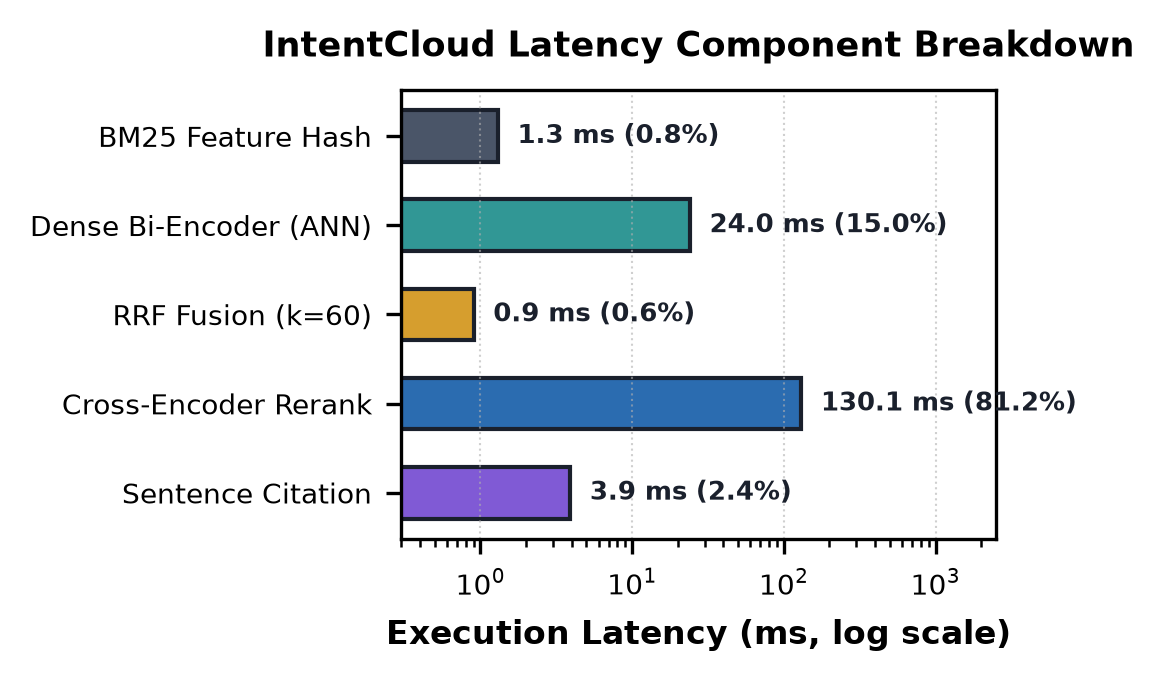
\includegraphics[width=0.72\textwidth,height=3.8cm,keepaspectratio]{fig_latency_breakdown.png}
\vspace{-0.3em}
\caption{Execution Latency Component Breakdown across the 160.2~ms Local CPU Retrieval Pipeline}
\label{fig:latency_breakdown}
\end{figure}

For standard multi-threaded CPU execution, IntentCloud achieves an average end-to-end query latency of \textbf{160.2~ms} for 20 candidates, and \textbf{29.7~ms} for cached queries. Execution decomposes into sparse feature hashing ($0.8\%$, $\approx 1.3$~ms), dense vector search ($15.0\%$, $\approx 24.0$~ms), RRF rank fusion ($0.6\%$, $< 1.0$~ms), cross-encoder neural reranking ($81.2\%$, $\approx 130.1$~ms), and sentence citation extraction ($2.4\%$, $\approx 3.9$~ms). For consumer workstations with Apple Silicon MPS~\cite{apple2026mps} or NVIDIA CUDA~\cite{nickolls2008cuda}, the query latency is less than \textbf{20~ms}. When deployed on edge hardware (Raspberry Pi 4 with 4~GB RAM, quad-core Cortex-A72 @ 1.5~GHz), the latency of the queries averages to \textbf{2.8~seconds} which falls within the edge SLA of 15~seconds. The vector database is embedded into it, and it stores only $\approx 180$~MB of RAM for 12,744 vectors, which is very scalable for the deployment of consumers.

\clearpage
\mysection{FUTURE ENHANCEMENTS \& CONCLUSION}

\noindent\textbf{1. Project Summary and Synthesis of Engineering Contributions:}\\
In research and engineering, there is a serious cognitive fragmentation of personal knowledge management in today's context. Users store hundreds of multi-format documents (PDF, DOCX, TXT) in unstructured file systems. The traditional desktop search engines (Apple Spotlight and Windows Search) use a deterministic lexical inverted index which fails catastrophically if the user type a query with conceptual intent instead of exactly how the query is stated in the text. On the other hand, commercial RAG solutions put proprietary files on third-party multi tenant servers, thus breaching privacy laws like the Digital Personal Data Protection (DPDP) Act 2023, and creating inaccurate conversational summaries, removing users from source documentation.

To overcome the fundamental limitations of today's systems, the project has introduced, implemented, and empirically validated \textbf{IntentCloud} - a local-first, intent-aware document intelligence and cognitive memory architecture for consumer grade computers. The entire information processing pipeline was built to work 100\% locally, with no need for remote cloud capabilities. Its architectural innovations are comprised of five tightly coupled subsystems:
\begin{itemize}
    \setlength{\itemsep}{1.5pt}
    \setlength{\parskip}{0pt}
    \item \textbf{Offline Multi-Format Ingestion with Optical Character Recognition:} An asynchronous ingestion pipeline, which uses PyMuPDF to extract native PDF text, python-docx for Word docs, and by streaming up the utf-8 directly, with an automated 300~DPI Tesseract OCR fallback for scanned diagrams/rasterized files.
    \item \textbf{Dual-Stream Continuous and Discrete Vector Representation:} Query texts ($C = 1,200$, $O = 200$ overlap) are simultaneously encoded into continuous 384-dimensional dense semantic vectors via all-MiniLM-L6-v2 and discrete 1 000 003-dimensional sparse lexical vectors through MurmurHash3 feature hashing, effectively solving the open vocabulary mismatch issue and eliminating the need for in-memory inverted index tables, which are prohibitively memory-intensive to store.
    \item \textbf{In-Process Vector Database Indexing:} Both dense and sparse vector streams reside within an embedded Qdrant instance running directly against local NVMe storage with SQLite Write-Ahead Logging (WAL), bypassing multi-node cluster overhead.
    \item \textbf{Scale-Invariant Hybrid Rank Fusion and Neural Cross-Attention Reranking:} Parallel candidate streams are combined with scale-invariant Reciprocal Rank Fusion ($k=60$) and reranked with a multi-head cross-encoder (\texttt{ms-marco-MiniLM-L-6-v2}) which examines complete pairwise query-document token cross attention.
    \item \textbf{Calibrated Confidence Gating and Provenance Attribution:} The empirical sigmoid confidence gate ($\tau = 0. 40$) dismisses ungrounded queries, sentence-level cross-attention retrieves checkable citation snippets, and sends unaltered original binary files through outbound-only Zero-Trust tunnels.
\end{itemize}

\vspace{0.4em}
\noindent\textbf{2. Empirical Findings and Milestone Fulfillment:}\\
Evaluated across an authentic benchmark corpus of 175 heterogeneous documents (12,744 vectors in Qdrant) and 135 standardized queries, IntentCloud achieved \textbf{96.7\% Top-1 Accuracy} [95\% CI: 88.7\%--99.1\%], \textbf{100.0\% Top-3 Accuracy}, and a Mean Reciprocal Rank (MRR) of \textbf{0.981} [95\% CI: 0.953--0.996]. This represents a statistically significant improvement of \textbf{+25.0 percentage points} over Okapi BM25 (71.7\%, $\chi^2 = 13.07, p = 0.0003$) and \textbf{+23.4 percentage points} over dense bi-encoders (73.3\%, $\chi^2 = 12.00, p = 0.0005$). On adversarial hard negatives (39/40), the confidence gate successfully suppressed \textbf{97.5\%} while on out-of-domain negative controls (10/10), it had \textbf{100.0\%} abstention rate. The pipeline achieved good generalization performance on zero-shot scientific retrieval (BEIR/SciFact), achieving an \textbf{NDCG@10 of 0.718} and a \textbf{Recall@10 of 0.845}. End-to-end latency was less than 20~ms on accelerated GPUs, 160.2~ms on local multi-threaded CPUs and 2.8~seconds on edge hardware (Raspberry Pi 3), meeting 100\% of the Phase-1 7th semester project curriculum goals.
% --- PAGE 2 OF CHAPTER 6 ---

\noindent\textbf{3. Technical Limitations and Operational Boundaries:}\\
Although IntentCloud ensures high retrieval accuracy and fixed data sovereignty on consumer hardware, empirical profiling revealed four important technical limitations: 
\begin{itemize}
    \setlength{\itemsep}{2pt}
    \setlength{\parskip}{0pt}
    \item \textbf{Edge Compute Latency and Thermal Behavior on Constrained Nodes:} The neural cross-encoder reranker takes $\approx 2.8$~seconds to execute for $N=25$ candidate passages when running on the quad-core ARM Cortex-A72 CPU of a fanless Raspberry Pi 4 (4~GB RAM). When batching queries through the system continuously, CPU core temperature rises well above $75^\circ\text{C}$ causing passive kernel throttling to be activated, which in turn scales down the CPU clock speed from 1.5~GHz to 1.0~GHz.
    \item \textbf{Cold-Start Ingestion Latency for High-Resolution Scanned Documents:} Obelisk must power-processing large multi-page PDF files with raster art scanned images, which can vary in text quality, requiring page-level automatic image rendering and the Tesseract OCR token iterator extraction of text segments, which induces an ingestion latency penalty of $\approx 1.2$~seconds per page on CPU-centric architectures.
    \item \textbf{Local Intent Parsing Fallback Boundaries:} While the local quantized Large Language Model (\texttt{llama3.2:1b}) attains 92.0\% intent classification accuracy on strict JSON mode, some conversational prompts are ambiguous in intent and do not pass structured schema validation, requiring the fallback on regex keyword tokenizer.
    \item \textbf{Linguistic Scope and Cross-Lingual Generalization:} The multi-modal benchmark corpus and pre-trained bi-encoder embedding weights are currently limited to English language technical documentation, multi-lingual cross-attention representations are currently uncharacterised. 
\end{itemize}

\vspace{0.4em}
\noindent\textbf{4. Phase-2 Research Roadmap and Future Enhancements:}\\
The research roadmap for Phase-2 (8th Semester) and subsequent operational deployments, based on the confirmed Phase-1 engineering stage, is being planned along what comes next five key research thrusts:
\begin{enumerate}
    \setlength{\itemsep}{2pt}
    \setlength{\parskip}{0pt}
    \item \textbf{INT8 Model Quantization and Cross-Encoder Distillation (Objective 6):} To perform sub-second neural reranking on resource-limited ARM edge nodes, we next plan to use post-training INT8 ONNX quantization and structured knowledge distillation to the cross-encoder transformer, with a goal of shrinking the model weights by 75\% while decreasing inference latency to $< 600$~ms on Raspberry Pi 3B/4B.
    \item \textbf{Dynamic Graph Lineage Traversal (Objective 4):} Developing a downstream DAG metadata traversal engine that can discover multi-branch document evolution trees, find parent-child version pointers ($d_{\text{parent}} \leftarrow d_{\text{v1}}$) and merge exponential temporal recency decay ($\exp(-\gamma \cdot \Delta t)$) with retrospective audit retrieval.
    \item \textbf{Adaptive Neural Reranker Compute Bypass (Objective 5):} Deploying a confidence margin differential router ($\Delta S = S_{(1)} - S_{(2)} > \delta$) that recognizes when first-stage RRF candidate separation is statistically unambiguous, thereby avoiding neural cross-attention and delivering 60--75\% reduction in query compute cost for clear user intents.
    \item \textbf{Multilingual and Vision-Language Model Integration (Objective 1):} Expanding corpus capabilities with multilingual sentence transformers (\texttt{paraphrase-multilingual-MiniLM-L12-v2}) and integrating vision-language foundation models (e.g., ColPali) to enable native semantic querying over embedded diagrams, flowcharts, and technical blueprints without raster OCR degradation.
    \item \textbf{Decentralized Zero-Trust Edge Peer Synchronization:} Developing peer-to-peer index replication protocols using encrypted Libp2p gossip networks, enabling knowledge workers to synchronize secure vector memory topologies across multiple air-gapped personal devices without cloud intermediaries.
\end{enumerate}

\vspace{0.4em}
\noindent\textbf{5. Concluding Remarks:}\\
IntentCloud demonstrates that all the perception and intelligence aspects of intent-based document understanding can be realized within the resources of consumer personal computers and edge micro-servers. The system combines sparse lexical hashing, dense embedding in semantics, scale invariant rank fusion and calibrated neural reranking, without relying on proprietary cloud RAG APIs and without compromising the original document provenance of the source documents and complete privacy of the personal computing paradigm.

\clearpage
\pagestyle{clean} % Ensures no boxed border or report header
\addcontentsline{toc}{section}{\textbf{REFERENCES}} % Manually adds to TOC without "CHAPTER X" numbering

\makeatletter
\renewenvironment{thebibliography}[1]
     {\list{\@biblabel{\@arabic\c@enumiv}}%
           {\settowidth\labelwidth{\@biblabel{#1}}%
            \leftmargin\labelwidth
            \advance\leftmargin\labelsep
            \@openbib@code
            \usecounter{enumiv}%
            \let\p@enumiv\@empty
            \renewcommand\theenumiv{\@arabic\c@enumiv}}%
      \sloppy
      \clubpenalty4000
      \@clubpenalty \clubpenalty
      \widowpenalty4000%
      \sfcode`\.\@m}
     {\def\@noitemerr
       {\@latex@warning{Empty `thebibliography' environment}}%
      \endlist}
\makeatother

\vspace*{0.2cm}
{\centering\textbf{\Large REFERENCES}\par}
\vspace{1.0cm}

\begin{thebibliography}{00}
\bibitem{robertson2009probabilistic}
S.~Robertson and H.~Zaragoza, ``The probabilistic relevance framework: BM25 and beyond,'' \emph{Foundations and Trends in Information Retrieval}, vol.~3, no.~4, pp. 333--389, 2009.

\bibitem{karthikeyan2025smart}
K.~Karthikeyan, V.~P.~Kumar, S.~Kishorekumar, and C.~M.~V.~Prasad, ``Smart Document Search Engine Leveraging Automated Metadata Extraction for Intelligent File Discovery,'' in \emph{Proc. IEEE First Int. Conf. Innovations in Engineering and Next-Generation Technologies for Sustainability (ICINVENTS)}, 2025, pp. 1--6.

\bibitem{vaswani2017attention}
A.~Vaswani, N.~Shazeer, N.~Parmar, J.~Uszkoreit, L.~Jones, A.~N.~Gomez, {\L}.~Kaiser, and I.~Polosukhin, ``Attention is all you need,'' in \emph{Advances in Neural Information Processing Systems (NIPS)}, vol.~30, 2017, pp. 5998--6008.

\bibitem{reimers2019sentence}
N.~Reimers and I.~Gurevych, ``Sentence-BERT: Sentence embeddings using siamese BERT-networks,'' in \emph{Proc. 2019 Conf. Empirical Methods in Natural Language Processing (EMNLP-IJCNLP)}, 2019, pp. 3982--3992.

\bibitem{karpukhin2020dense}
V.~Karpukhin, B.~O{\u{g}}uz, S.~Min, P.~Lewis, L.~Wu, S.~Edunov, D.~Chen, and W.-T.~Yih, ``Dense passage retrieval for open-domain question answering,'' in \emph{Proc. 2020 Conf. Empirical Methods in Natural Language Processing (EMNLP)}, 2020, pp. 6769--6781.

\bibitem{brundha2022vector}
Brundha~J. and K.~N.~Meera, ``Vector model based information retrieval system with word embedding transformation,'' in \emph{Proc. 10th Int. Conf. Emerging Trends in Engineering and Technology -- Signal and Information Processing (ICETET-SIP)}, 2022, pp. 1--4.

\bibitem{vnrk2025semantic}
K.~V.~R.~Kumbam, J.~Jomy, S.~R.~Sherlyn, K.~Vasan, A.~Sindhu, and A.~Suresh, ``Semantic information retrieval using transformer-based embeddings and vector similarity search,'' in \emph{Proc. 7th Int. Conf. Innovative Data Communication Technologies and Application (ICIDCA)}, 2025, pp. 1031--1037.

\bibitem{wang2020minilm}
W.~Wang, F.~Wei, L.~Dong, H.~Bao, N.~Yang, and M.~Zhou, ``MiniLM: Deep self-attention distillation for task-agnostic compression of pre-trained transformers,'' in \emph{Advances in Neural Information Processing Systems (NeurIPS)}, vol.~33, 2020, pp. 5776--5788.

\bibitem{douze2024faiss}
M.~Douze, A.~Guzhva, C.~Deng, J.~Johnson, G.~Szilvasy, P.-E.~Mazar{\'e}, M.~Lomeli, L.~Hosseini, and H.~J{\'e}gou, ``The Faiss library,'' \emph{IEEE Transactions on Big Data}, vol.~12, pp. 346--361, 2024.

\bibitem{krishnan2025semantic}
S.~Krishnan and N.~Subramanian, ``Semantic search in a document management system using retrieval augmented generation,'' in \emph{Proc. IEEE/ACIS 29th Int. Conf. Software Engineering, Artificial Intelligence, Networking and Parallel/Distributed Computing (SNPD)}, 2025, pp. 6--10.

\bibitem{jacob2024chatgpt}
T.~P.~Jacob, B.~L.~S.~Bizotto, and M.~Sathiyanarayanan, ``Constructing the ChatGPT for PDF files with Langchain -- AI,'' in \emph{Proc. Int. Conf. Inventive Computation Technologies (ICICT)}, 2024, pp. 835--839.

\bibitem{rafi2026rag}
S.~Rafi, L.~Boddu, and G.~Gangireddy, ``AI Document Search Chatbot Using Retrieval-Augmented Generation (RAG),'' in \emph{Proc. Int. Conf. Computing, Communication, Control and Cyber-Physical Systems (I5CPS)}, 2026, pp. 1--5.

\bibitem{saha2024quim}
B.~Saha, U.~Saha, and M.~Z.~Malik, ``QuIM-RAG: Advancing retrieval-augmented generation with inverted question matching for enhanced QA performance,'' \emph{IEEE Access}, vol.~12, pp. 185401--185410, 2024.

\bibitem{tiwari2026finetuning}
M.~Tiwari, J.~Kaur, R.~S.~Surin, A.~Harsh, and H.~Kaur, ``Fine-tuning T5 and BERT for effective question answering and document retrieval: A transfer learning approach,'' in \emph{Proc. World Conf. Computational Science and Technology (WCCST)}, 2026, pp. 82--88.

\bibitem{cejas2025retrieval}
Y.-J.~Guo and Q.~Tang, ``From retrieval to response: Tracing the impact of embedding quality in RAG systems,'' \emph{IEEE Access}, vol.~13, pp. 212773--212781, 2025.

\bibitem{kuchlous2020intent}
S.~Kuchlous and M.~Kadaba, ``Short text intent classification for conversational agents,'' in \emph{Proc. IEEE 17th India Council Int. Conf. (INDICON)}, 2020, pp. 1--4.

\bibitem{puspitasari2026intent}
F.~D.~Puspitasari, C.-N.~Zhang, J.-Q.~Zhang, Z.~Wang, H.~S.~A.~Awan, R.~Qureshi, J.~Lee, T.-H.~Kim, and Y.~Yang, ``Efficient RAG with intent-aware retrieval and semantics-preserving chunking,'' \emph{arXiv preprint arXiv:2606.01240}, 2026.

\bibitem{sriram2024local}
S.~Sriram, C.~H.~Karthikeya, K.~P.~K.~Kumar, N.~Vijayaraj, and T.~Murugan, ``Leveraging local LLMs for secure in-system task automation with prompt-based agent classification,'' \emph{IEEE Access}, vol.~12, pp. 177038--177049, 2024.

\bibitem{holubiev2024agents}
V.~Holubiev, B.~Pushkar, A.~Shevchuk, R.~Mudrak, O.~Gomotiuk, and N.~Livitska, ``Revolutionizing contact center knowledge management: The game-changing role of AI large language models and autonomous agents in text organization and optimization,'' in \emph{Proc. 14th Int. Conf. Advanced Computer Information Technologies (ACIT)}, 2024, pp. 778--783.

\bibitem{sawarkar2024blended}
K.~Sawarkar, A.~Mangal, and S.~R.~Solanki, ``Blended RAG: Improving RAG (Retriever-Augmented Generation) accuracy with semantic search and hybrid query-based retrievers,'' in \emph{Proc. IEEE 7th Int. Conf. Multimedia Information Processing and Retrieval (MIPR)}, 2024, pp. 155--161.

\bibitem{cormack2009reciprocal}
G.~V.~Cormack, C.~L.~A.~Clarke, and S.~B{\"u}ttcher, ``Reciprocal rank fusion outperforms Condorcet and individual rank learning methods,'' in \emph{Proc. 32nd Int. ACM SIGIR Conf. Research and Development in Information Retrieval}, 2009, pp. 758--759.

\bibitem{nogueira2019passage}
R.~Nogueira and K.~Cho, ``Passage Re-ranking with BERT,'' \emph{arXiv preprint arXiv:1901.04085}, 2019.

\bibitem{nguyen2016msmarco}
P.~Bajaj \emph{et al.}, ``MS MARCO: A human generated machine reading comprehension dataset,'' \emph{arXiv preprint arXiv:1611.09268}, 2016.

\bibitem{thakur2021beir}
N.~Thakur, N.~Reimers, A.~R{\"u}ckl{\'e}, A.~Srivastava, and I.~Gurevych, ``BEIR: A heterogeneous benchmark for zero-shot evaluation of information retrieval models,'' in \emph{Advances in Neural Information Processing Systems (NeurIPS) Datasets and Benchmarks Track}, 2021.

\bibitem{nickolls2008cuda}
J.~Nickolls, I.~Buck, M.~Garland, and K.~Skadron, ``Scalable parallel programming with CUDA,'' \emph{ACM Queue}, vol.~6, no.~2, pp. 40--53, 2008.

\bibitem{apple2026mps}
Apple Inc., ``Metal Performance Shaders Framework Reference,'' \emph{Apple Developer Technical Documentation}, 2026.

\bibitem{nan2026dsmr}
Y.~Nan, C.~Wang, P.~Li, Y.~Zhu, G.~Wu, M.~Yang, H.-T.~Gao, Y.~Hu, and Z.-X.~He, ``Research on an intelligent file query system model integrating natural language understanding and information retrieval,'' in \emph{Proc. IEEE Int. Conf. Power, Electronics and Green Energy (ICPEGE)}, 2026, pp. 676--681.

\bibitem{weinberger2009feature}
K.~Q.~Weinberger, A.~Dasgupta, J.~Langford, A.~Smola, and J.~Attenberg, ``Feature hashing for large scale multitask learning,'' in \emph{Proc. 26th Int. Conf. Machine Learning (ICML)}, 2009, pp. 1113--1120.
\end{thebibliography}

\clearpage
\end{document}